\chapter{Cross-tissue comparison of chromatin accessibility, gene expression signature and immunophenotypes in PsA}
\chaptermark{Cross-tissue comparison analysis in PsA}
\label{ch:Results3}


%%%%%%%%%%%%%%%%%%%%%%%%%%%%%%%%%%%%%%%%%%%%%%%%%%
\section{Introduction}
%
The techniques to generate the scRNA-seq data have also evolved and SmartSeq2 and 10X Chromium are the two main 
%%%%%%%%%%%%%%%%%%%%%%%%%%%%%%%%%%%%%%%%%%%%%%%%%%
\section{Results}
%

\subsection{PsA patients cohort description and datasets}
In this study peripheral blood (PB) and SF were collected from a cohort of six PsA patients, with equal numbers of males and females (Table \ref{tab:PSA_cohort_metadata}). All the patients presented oligoarticular joint affection and had been first diagnosed with psoriasis. The cohort presented a mean of 1.5 tender or swollen affected joints (TJC66 and SJC66), which is characteristic of the oligoarticular form of disease (involving one or few joint and joint pain of xxxx. Regarding global assessment, the mean scores for the patient and physician evaluation were X and 3, respectively, in a scale of 1 to 5. These four measurements including joints and global assessment compose the PsARC disease activity scores, used by clinicians as the main indicator of response to treatment by recommendation of the National Institute for Health and Care Excellence (NICE)(Chapter \ref{ch:Intro}). 

The mean age of the cohort at the time of diagnosis was 44.3 years old and the mean disease duration 8.8 years. Interestingly, PsA1728 was diagnosed at a later age compared to the other patients in the cohort (late PsA onset clinical significance??). Moreover, C-reactive protein (CRP) levels, other marker of inflammation, presented an average of 17.45 mg/L and was particularly higher in PSA1719 and PSA1728 compared to the other patients. At the time of sample recruitment all the PsA patients were naive for treatment and only PSA1505 had been on MTX therapy in the past for xxx months/years (how many years ago?). Post-visit, most of the patients qualified for TNAi biologic therapy xxxx.


%
\begin{landscape}
\begin{center}
\begin{longtable}[ht]{c c c c c c c c}
%{p{.15\textheight} p{.15\textheight} p{.25\textheight} p{.25\textheight} p{.15\textheight} p{.15\textheight} p{.15\textheight}}
\caption[Description of PsA patients cohort recruitment and metadata.]{\textbf{Description of PsA patients cohort recruitment and metadata.}. PsARC disease activity score is composed of tender joint count 66 (TJC66) and swollen joint count 66 (SJC66), joint pain (4 point score) and self-patient and physician global assessment (5 point score). Joint pain and global assessment use a likert scale based on questionnaire answers that measure the level of agreement with each of statements included. C-reactive protein (CRP).}
\label{tab:PSA_cohort_metadata} \\
\toprule
\textbf{ Sample ID} & \textbf{Sex} & \textbf{Age} & \textbf{Disease duration} & \textbf{Type} &\textbf{TJC66/SJC66}  & \textbf{Physician } & \textbf{CRP} \\
& & \textbf{diagnosis} & \textbf{(months)} & &  & \textbf{assessment} & \textbf{(mg/L)} \\
\midrule
\midrule
PSA1718 & Female & 17 & 180 & Oligo  & 2/2 & 3 & 6 \\
PSA1719	& Male &	33 & 24	 & Oligo &	1/1 &	3 & 36.6 \\           
PSA1607 &	Male & 42 & 108 &	Oligo &	1/1	& 4 & 8 \\
PSA1728	& Female & 72	& 48 & Oligo & 2/2 & 3 & 43.2 \\
PsA1801	& Female & 53 & 168 & Oligo & 2/2 &	3 & 9.9 \\
PsA1505 & Male & 35 &	108 & Oligo & 1/1 & 2 & 1 \\	
\midrule
Total		& $-$	&	44.3 & 106 & $-$ & 1.5/1.5 & 3 & 17.45 \\																			
\bottomrule
\medskip
\end{longtable}
\end{center}
\end{landscape}

%\clearpage

For each of the patients, paired data in PB and SF was generated from bulk mononuclear cells or specific isolated cell types of interest (detailed in Table \ref{tab:PSA_datasets_per_sample} and Chapter \ref{ch:Mat}). Due to project contrains, ATAC-seq, PCR gene expression array, scRNA-seq and mass cytometry were not generated for all six individuals in the cohort. 

\begin{table}[htbp]
%\setlength{\tabcolsep}{20pt} only to stretch the columns if you want
%\renewcommand{\arraystretch}{1.5}
\centering
\begin{tabular}{@{} c c c c c}
\toprule
\textbf{Sample ID} & \textbf{\% FAST-ATAC} & \textbf{RNA PCR array} & \textbf{scRNA-seq} & \textbf{Mass cytometry} \\
\midrule
\midrule
PSA1718 & Yes & Yes & No & Yes\\
PSA1719 & Yes & Yes & No & Yes\\
PSA1607 & Yes & No & Yes & Yes\\
PSA1728 & No & Yes & No & No\\
PSA1801 & No & No & Yes & No\\
PSA1605 & No & No & Yes & No\\
\bottomrule
\end{tabular}
\medskip %gap
\caption[Datasets generated for the PsA cohort samples]{\textbf{Datasets generated for the PsA cohort samples.} Four types of data were generated in a paired way between PB and SF from the same individual. The available data sets vary between individuals due to project constrains. FAST-ATAC data was generated for CD14$^+$, mCD4$^+$,mCD8$^+$ and NK cells. RNA expression by PCR array was performed for CD14$^+$, mCD4$^+$ and mCD8$^+$. scRNA-seq data was generated using 10X technology in bulk PBMCs, bulk SFMCs and sorted mCD4$^+$ and mCD8$^+$ isolated from both tissues.}
\label{tab:PSA_datasets_per_sample}
\end{table}
\bigskip %bigger space


\subsection{The chromatin accessibility landscape in SF and PB immune cells}

\subsubsection{Quality control of open chromatin regions}
The twenty four FAST-ATAC PsA samples from four different cell types and two tissues (PB and SF) were sequenced to a median of 158M reads (79M paired-end) per sample. After filtering for low quality mapping, duplicates and MT reads, the median total number of reads ranged between 46.6 and 70.2 M reads, upon cell type (Figure \ref{figure:PsA_FAST_ATAC_QC} a).  Overall, MT and duplicated reads accounted for a median between 40 to 62.2\% of the total number of reads depending on cell type (Figure \ref{figure:PsA_FAST_ATAC_QC} b) and importantly contributing to the loss of reads FAST-ATAC. The final number of reads remaining after filtering was inversely related to the percentage of MT and duplicated reads identified. For example, mCD14$^+$ and mCD8$^+$ presented the lowest median of total number of reads after filtering concomitantly with the greatest percentage of combined MT and duplicated reads. 
%As previously mentioned, the MT DNA in ATAC-seq is one of the main sources of read loss, which is more accessible to the Tn5 transposase due to the absence of nucleosomes. Although the FAST-ATAC protocol represented an improvement, the percentage of MT reads across amongst all the samples ranged between 2.1 and 25.4\%. Similarly, despite initial optimisation of the number of PCR cycles used in the library amplification, the duplicated reads still represented between 22.9 to 55\% of the total number sequenced reads.

Regarding sample quality, TSS enrichment analysis showed differences in the levels of background noise across cell types and highlighted the variability of FAST-ATAC performance (Figure \ref{figure:PsA_FAST_ATAC_QC} c). A trend towards greater TSS enrichment in PB samples compared to SF was observed in all four cell types. mCD4$^+$ and mCD8$^+$ presented the best signal-to-noise ratios, with median of 19.1 and 23.1 fold enrichment, respectively. In contrast, NK was the cell type with the lowest TSS enrichment values. Particularly, the fold enrichment for PSA1719 and PSA1607 were 7.3 and 6.2, respectively, both just above the 6 to 10 acceptable range from ENCODE. If bigger cohort size was available, dropping these two samples from the differential analysis would be beneficial since high background levels can reduce the power of this approach. 

 
\bigskip
\begin{figure}[H]
\centering
\begin{subfigure}[b]{0.48\textwidth}
\centering 
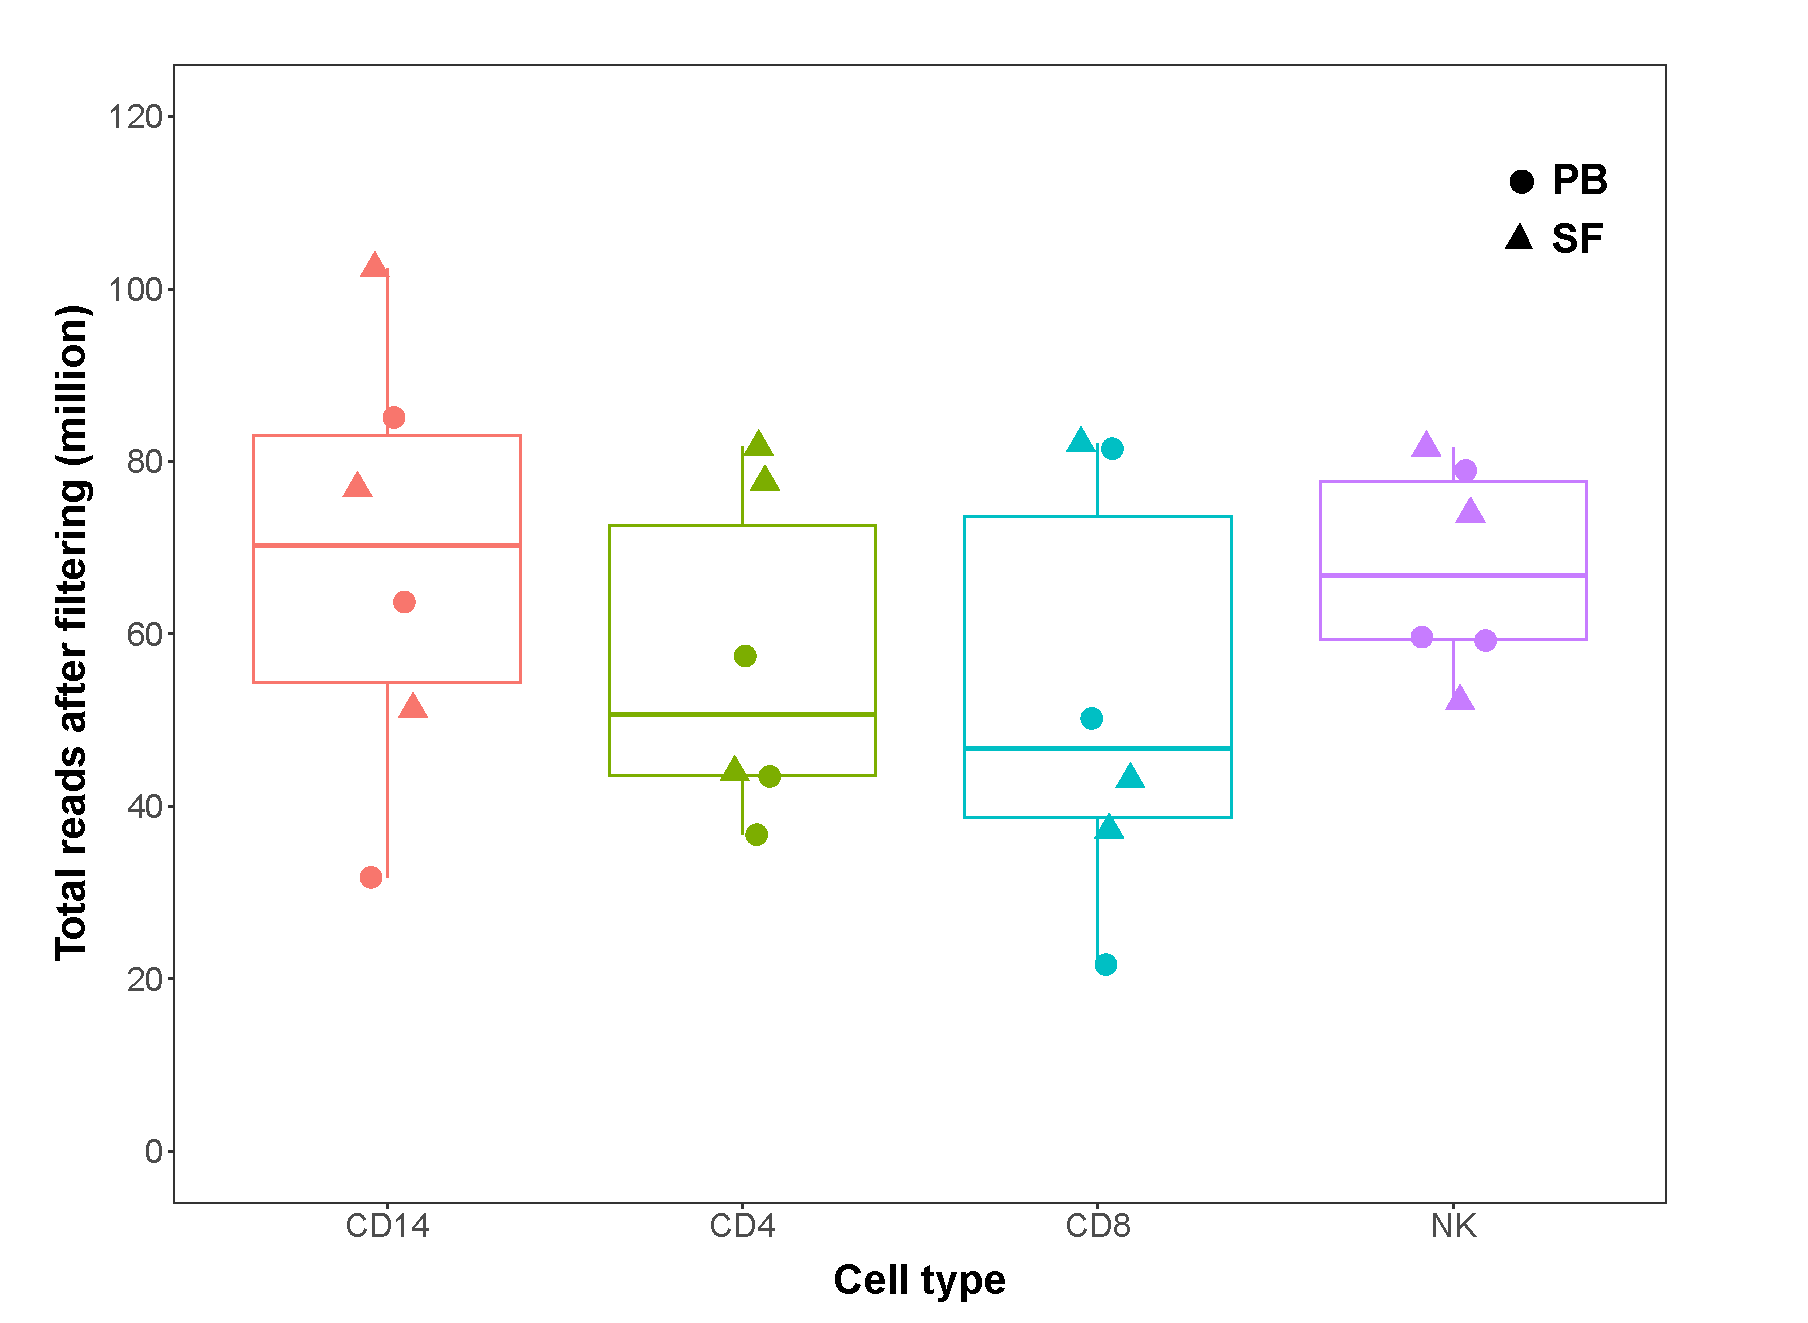
\includegraphics[width=\textwidth]{./Results3/pdfs/ATAC_PSA_total_filtered_reads_boxplot}
\caption{}
\end{subfigure}
~
\begin{subfigure}[b]{0.48\textwidth}
\centering 
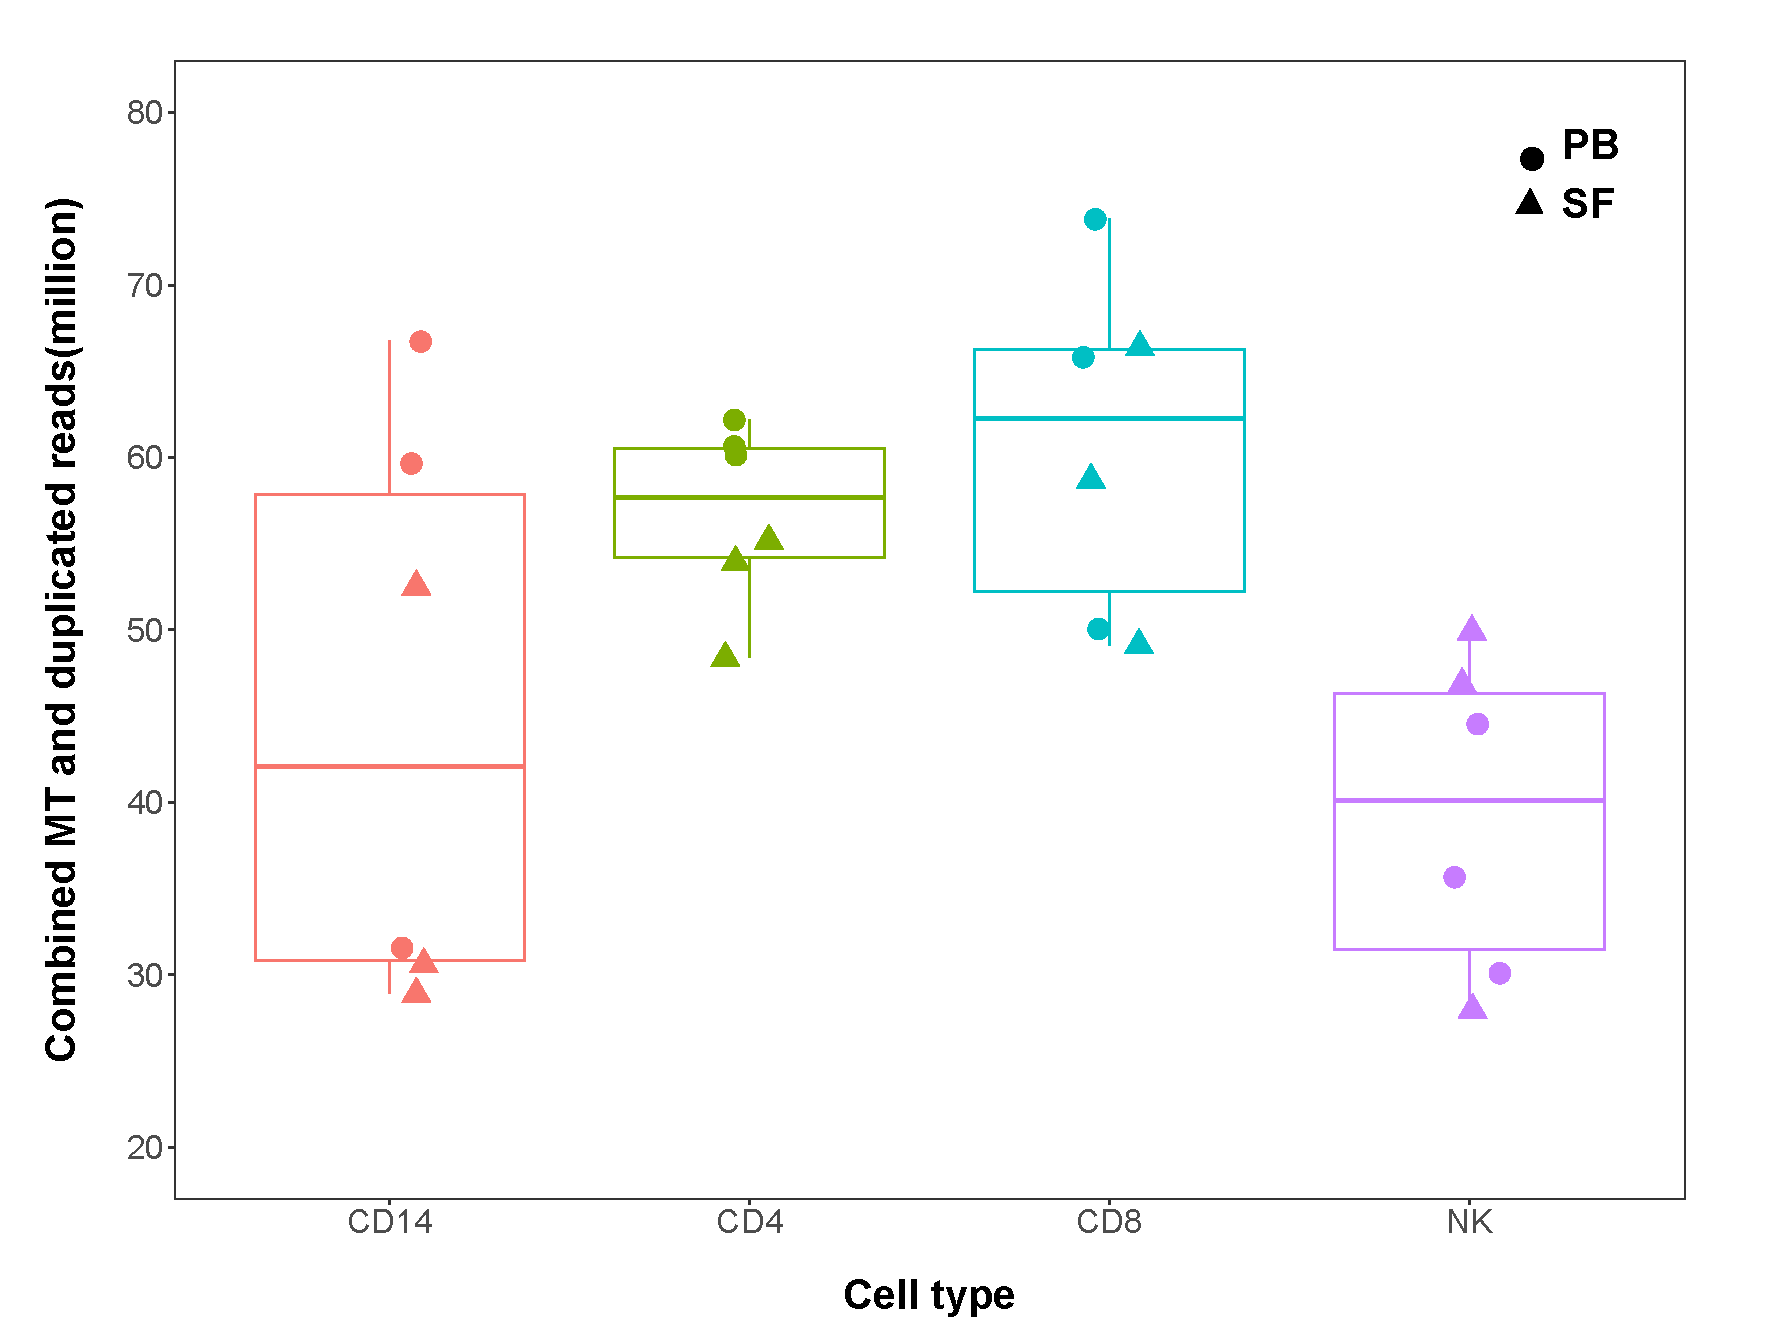
\includegraphics[width=\textwidth]{./Results3/pdfs/ATAC_PSA_pcnt_dups_and_MT_reads_boxplot}
\caption{}
\end{subfigure}
~
\begin{subfigure}[b]{0.48\textwidth} 
%the [b] prevents offset in subcaptions
\centering
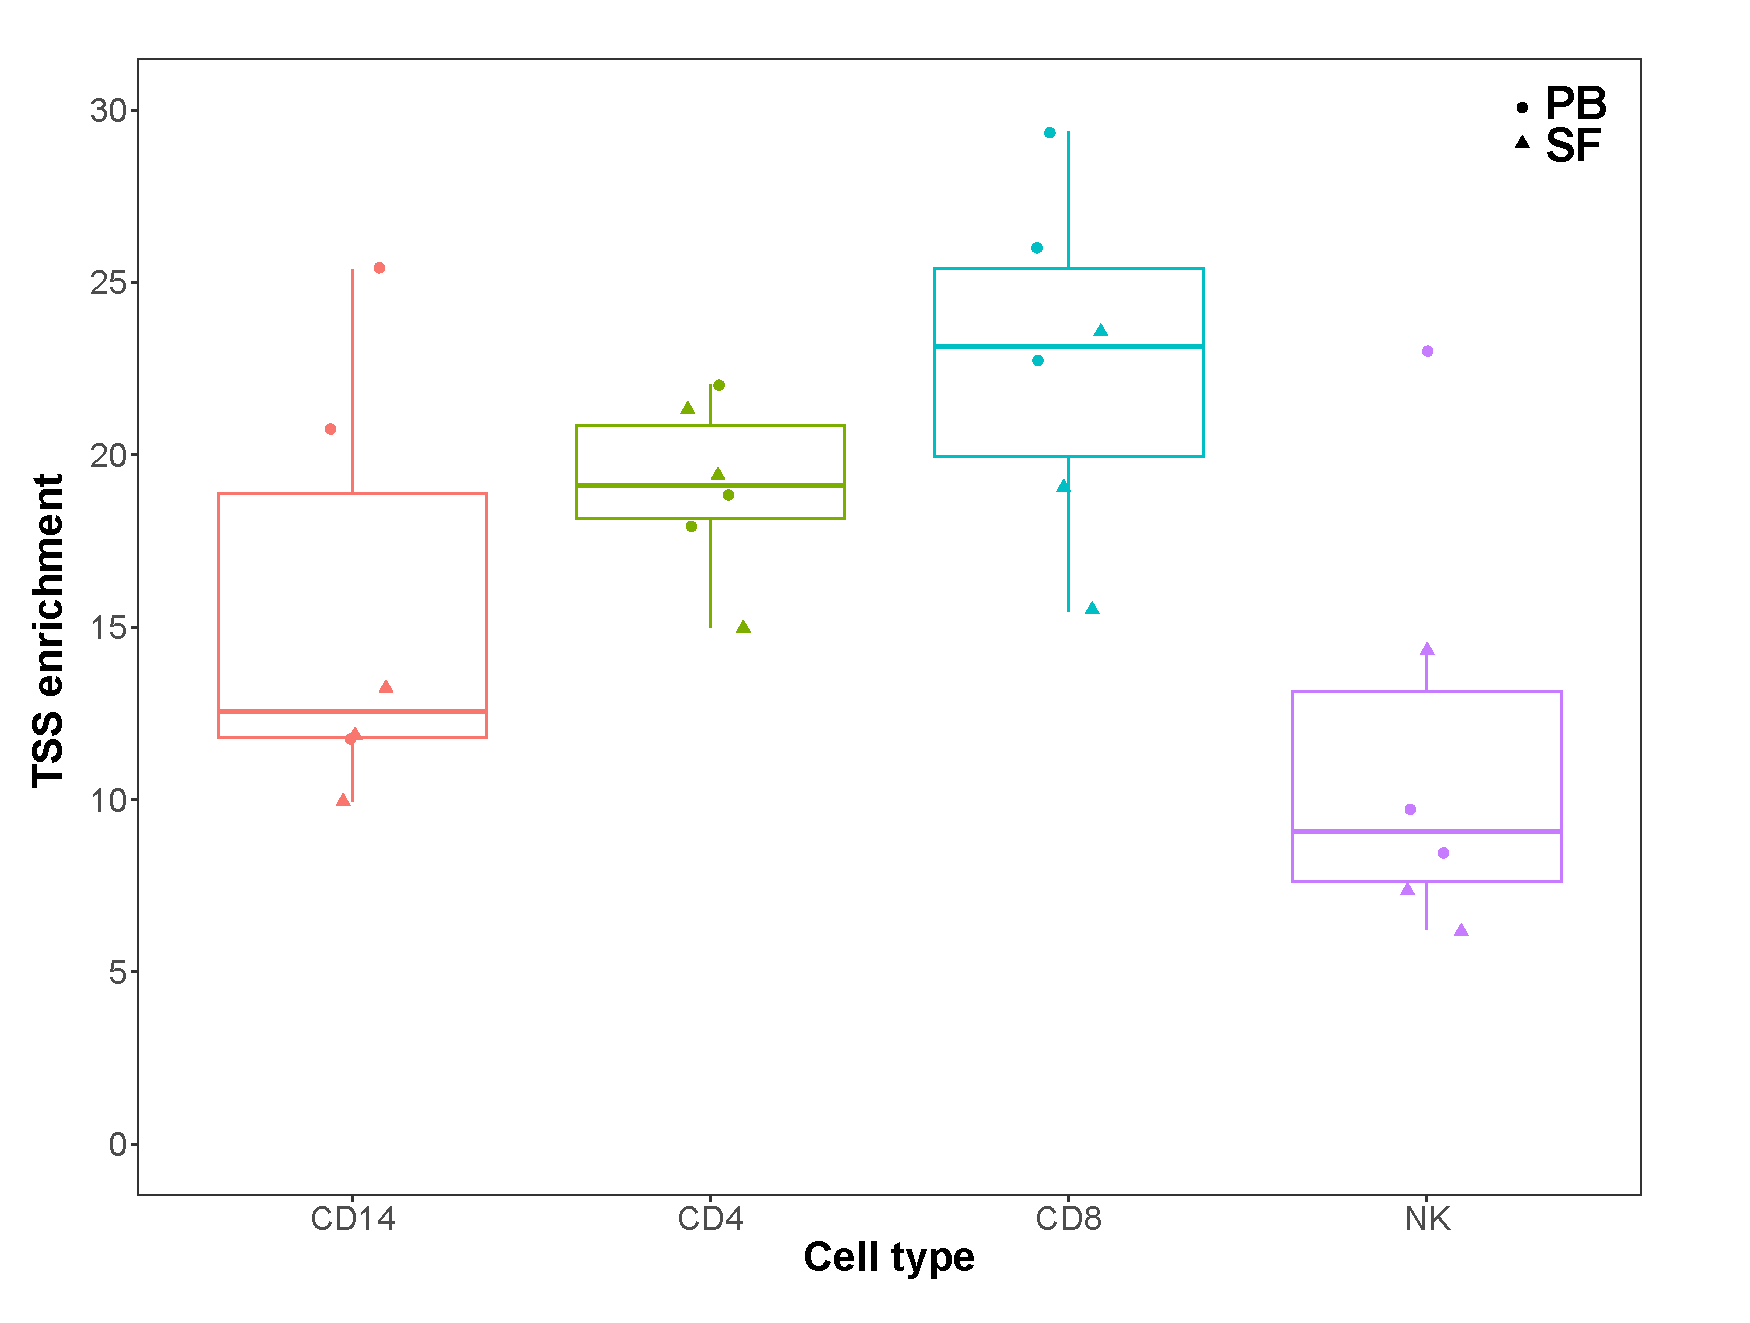
\includegraphics[width=\textwidth]{./Results3/pdfs/ATAC_PSA_all_TSS_max_per_cell_type}%
\caption{}
\end{subfigure}
\begin{subfigure}[b]{0.48\textwidth} 
%the [b] prevents offset in subcaptions
\centering
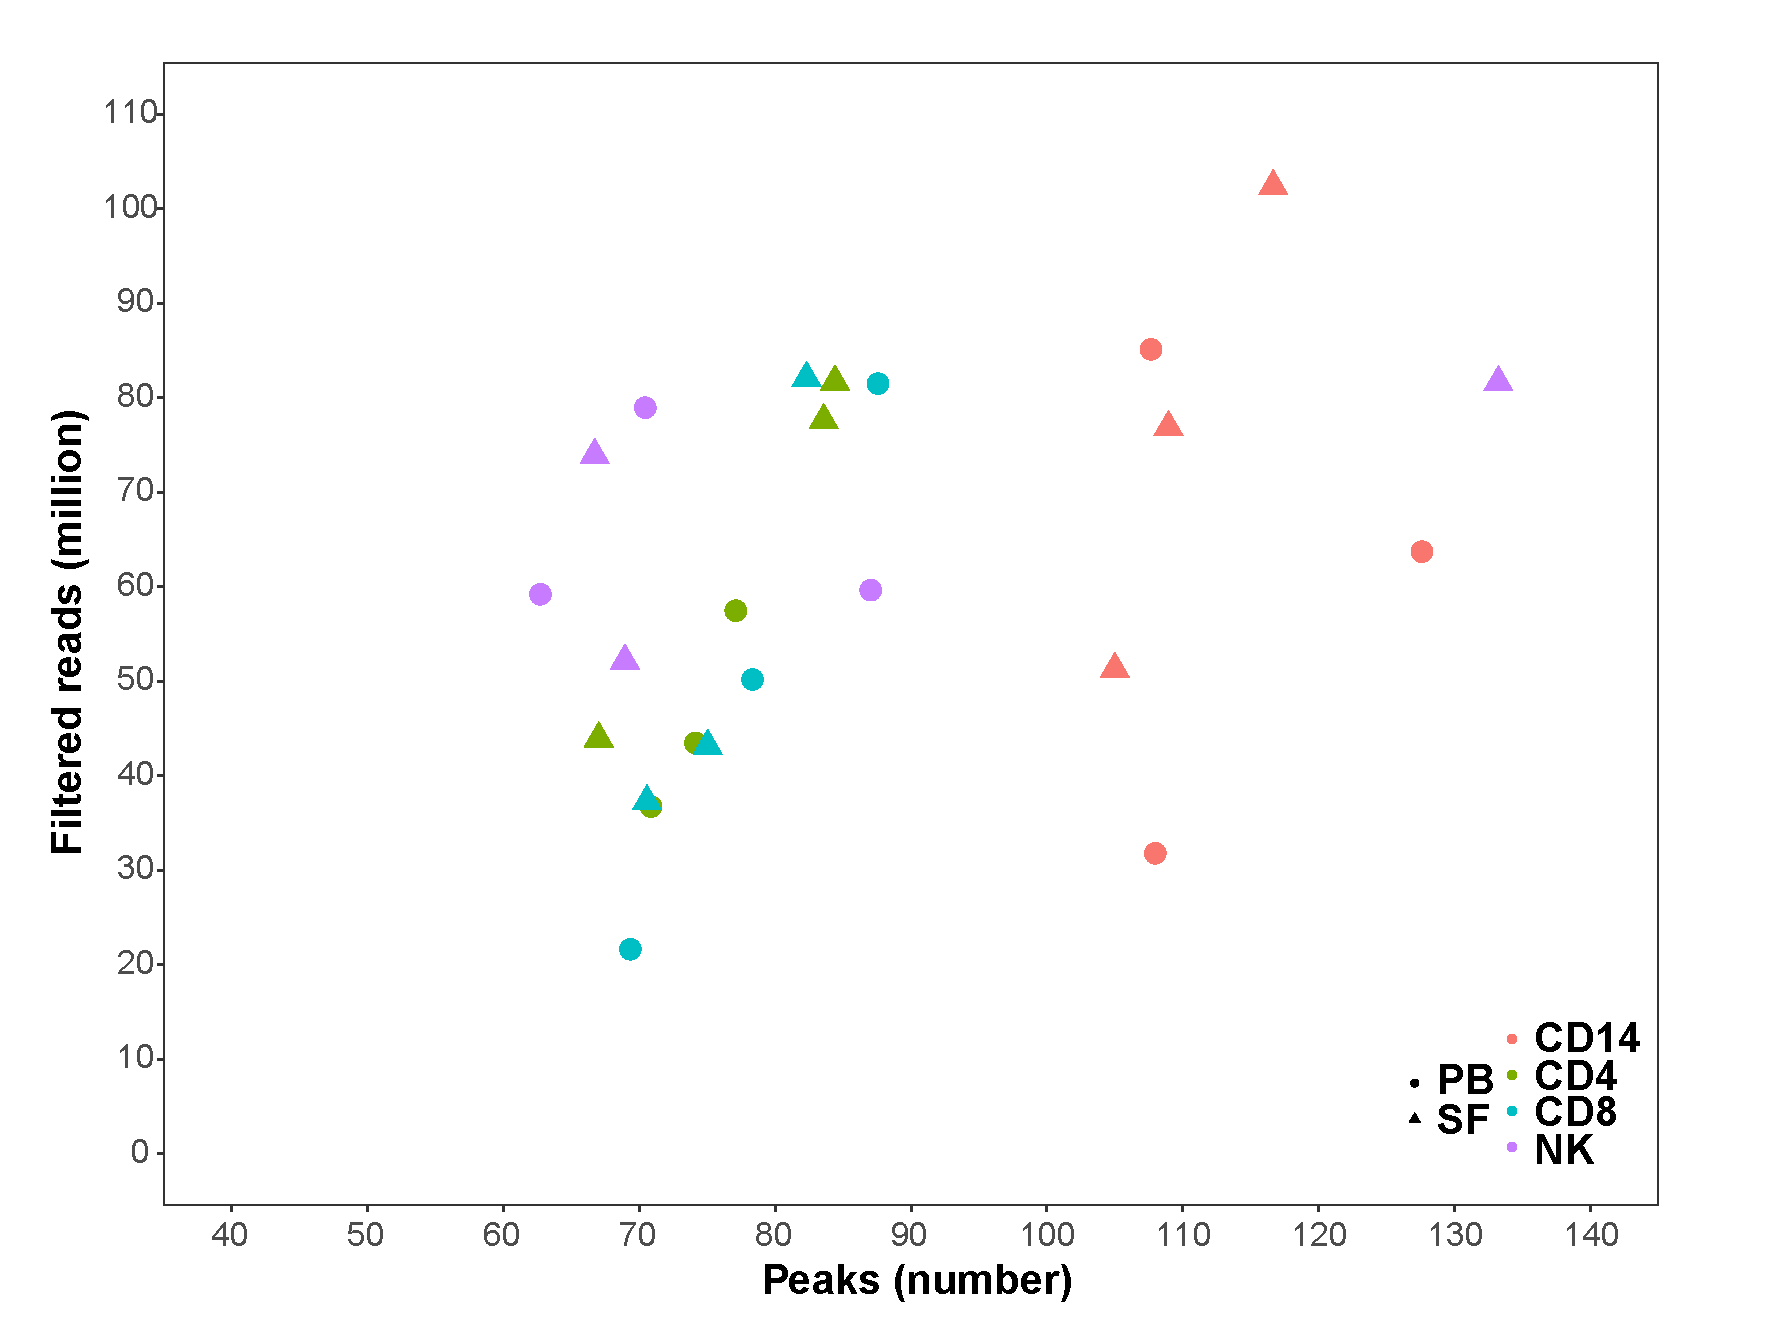
\includegraphics[width=\textwidth]{./Results3/pdfs/ATAC_PSA_all_peaks_vs_num_reads}%
\caption{}
\end{subfigure}
\caption[QC of FAST-ATAC PsA samples in four cell types]{\textbf{QC of FAST-ATAC PsA samples in four cell types}. }
\label{figure:PsA_FAST_ATAC_QC}
\end{figure}

When identifying open chromatin regions by peak calling using standard filtering (FDR$<$0.01), the number of accessible regions per sample ranged between $\sim$62$x10^3$ to $\sim$133$x10^3$ (Figure \ref{figure:PsA_FAST_ATAC_QC} d). A positive correlation between the number of called peaks and number of reads after filtering could be observed in the data. For example, CD14$^+$ was the cell type with greatest number of called peaks (108.4$x10^3$) as well as the greater median of reads remaining after filtering when compared to the other three cell types (Figure \ref{figure:PsA_FAST_ATAC_QC} a). Overall, appropriate number of peaks were called in all samples and no concerning outliers were identified.
%For example, the two NK samples with the greatest TSS enrichment (PSA1718 SF and PB) showed larger number of called peaks when compared to the other NK samples with similar number of reads but lower quality measured by TSS enrichment. This observation was consistent with the correlation between sample quality and the number of identified accessible chromatin regions previously demonstrated in Chapter \ref{ch:Results1}. 



\subsubsection{Open chromatin reflects cell type specificity and functional relevance}
To determine the ability of in house pipeline open chromatin to recapitulate cell type specificity in the PsA sample cohort, a combined master list including all four cell types and the two tissues was built. Following Chapter \ref{ch:Mat} and Chapter \ref{ch:Results1}, the combined master list contained open chromatin regions identified in at least 30\% of the samples (7 out of 24 samples), regardless cell type and tissue to avoid any bias. PCA analysis based on chromatin accessibility showed that most of the samples variability (PC1 65.6\% of the variability) correlated with cell type, leading to sample separation in four cluster (Figure \ref{figure:PsA_FAST_ATAC_PCA}. As expected, the myeloid (CD14$^+$ monocytes) and lymphoid (mCD4$^+$ and mCD8$^+$) clusters were the ones presenting greatest differences in chromatin accessibility pattern whereas the mCD4$^+$ and mCD8$^+$ clusters were the most similar between them. Modest clear separation between SF and PB samples was found in the mCD4$^+$, mCD8$^+$ and NK clusters.

\begin{figure}[H]
\centering
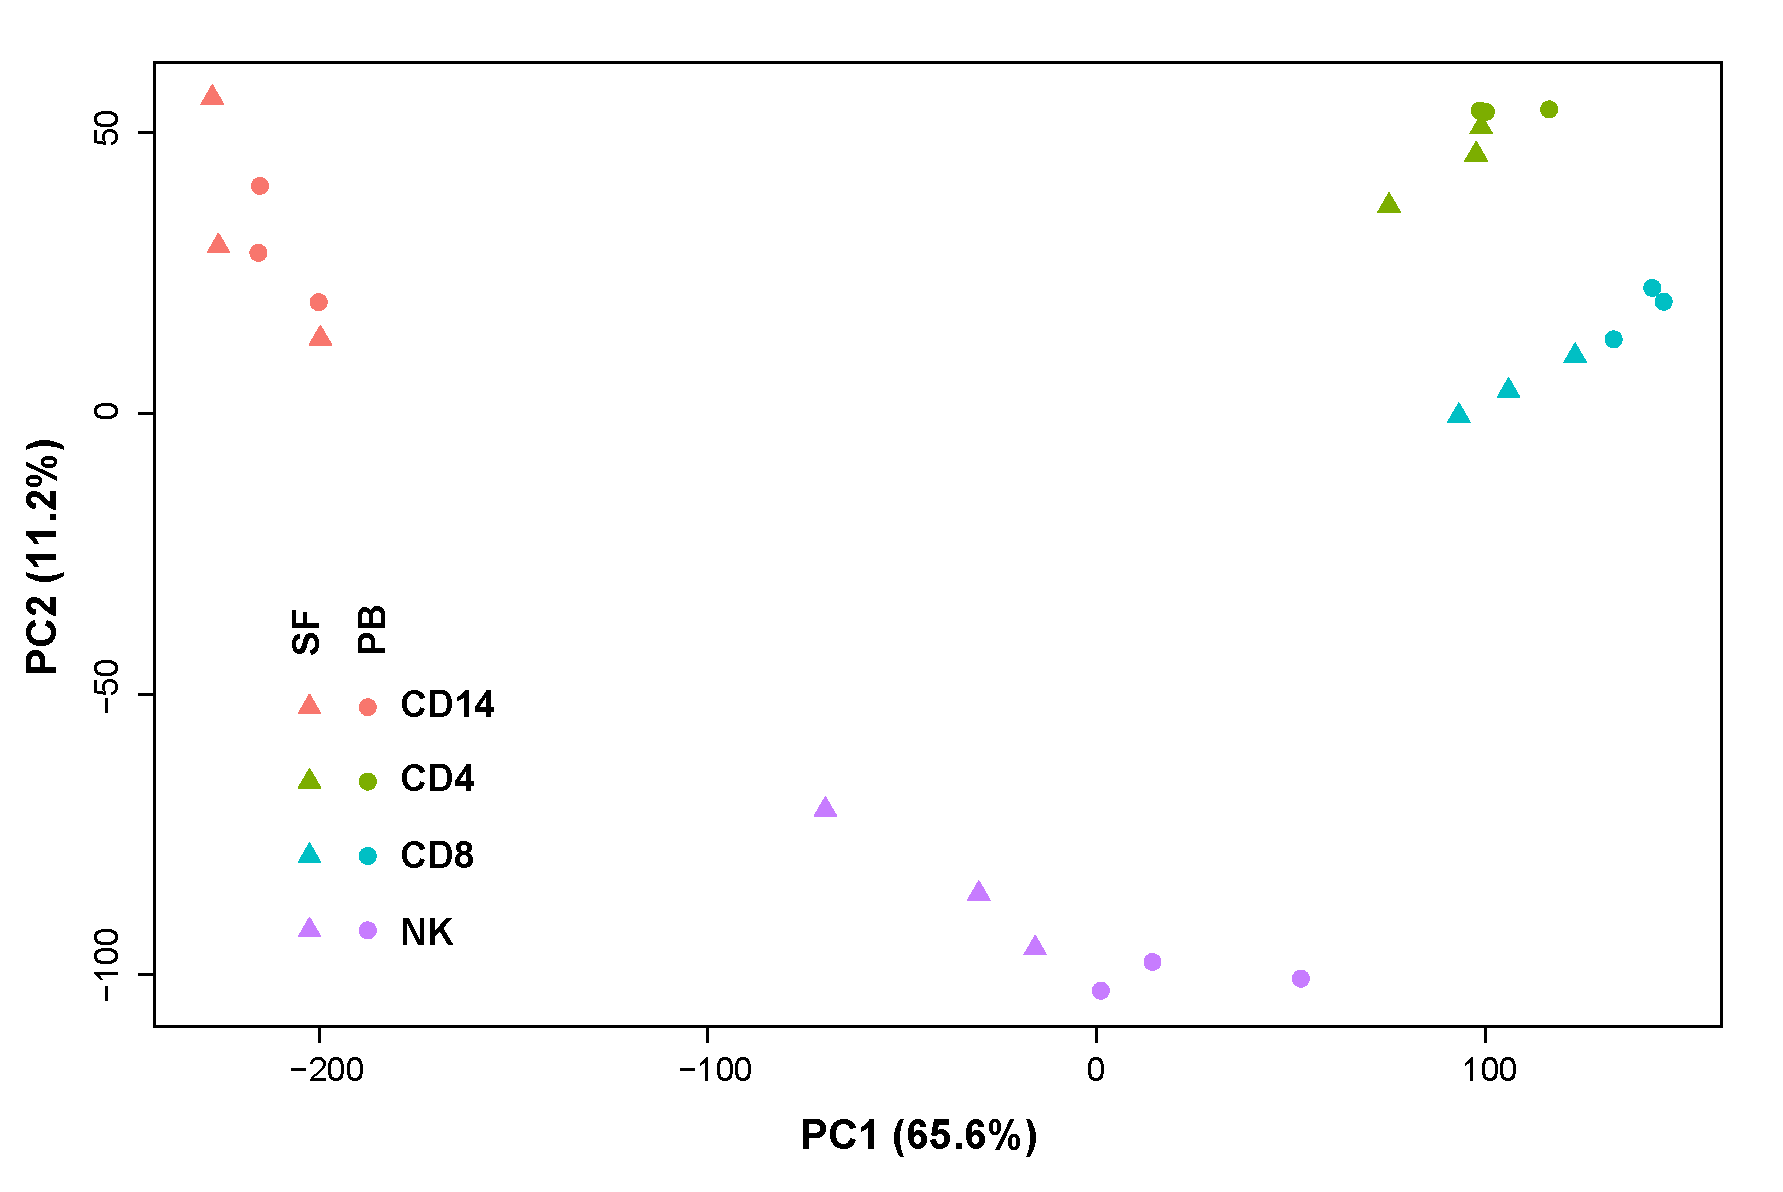
\includegraphics[width=0.7\textwidth]{./Results3/pdfs/ATAC_PSA_all_DESEq2_PCA}
\caption[Combined PCA analysis of all four cell types isolated from blood and SF.]{\textbf{Combined PCA analysis of all four cell types isolated from blood and SF.}}
\label{figure:PsA_FAST_ATAC_PCA}
\end{figure}

The ability to capture putative regulatory regions within the identified accessible chromatin in the four cell types was also explored. Enrichment analysis of different eQTL publicly available data sets for the combined chromatin accessibility master list was performed. Amongst the GTEx eQTL data, the greatest (z-score) and most significant (-log$_10$FDR) enrichment was found for the venous blood data set (red dot), consistently with the cell types included in the study (Figure \ref{figure:PsA_FAST_ATAC_eQTL_enrichment} a). Moreover, the greatest enrichments of immune-related cells in the accessible chromatin regions were found for CD14$^+$ monocytes (importantly unstimulated, LPS 2h and IFN-$\gamma$ 24h) followed by mCD8$^+$ T cells (Figure \ref{figure:PsA_FAST_ATAC_eQTL_enrichment} b). Interestingly, the B cells eQTLs were the least enriched in the chromatin accessibility data, consistently with the limited relevance of this cell type in psoriasis and PsA pathophysiology as well as the absence of this cell type amongst the ones included in the study.       

\bigskip
\begin{figure}[H]
\centering
\begin{subfigure}[b]{0.7\textwidth}
\centering 
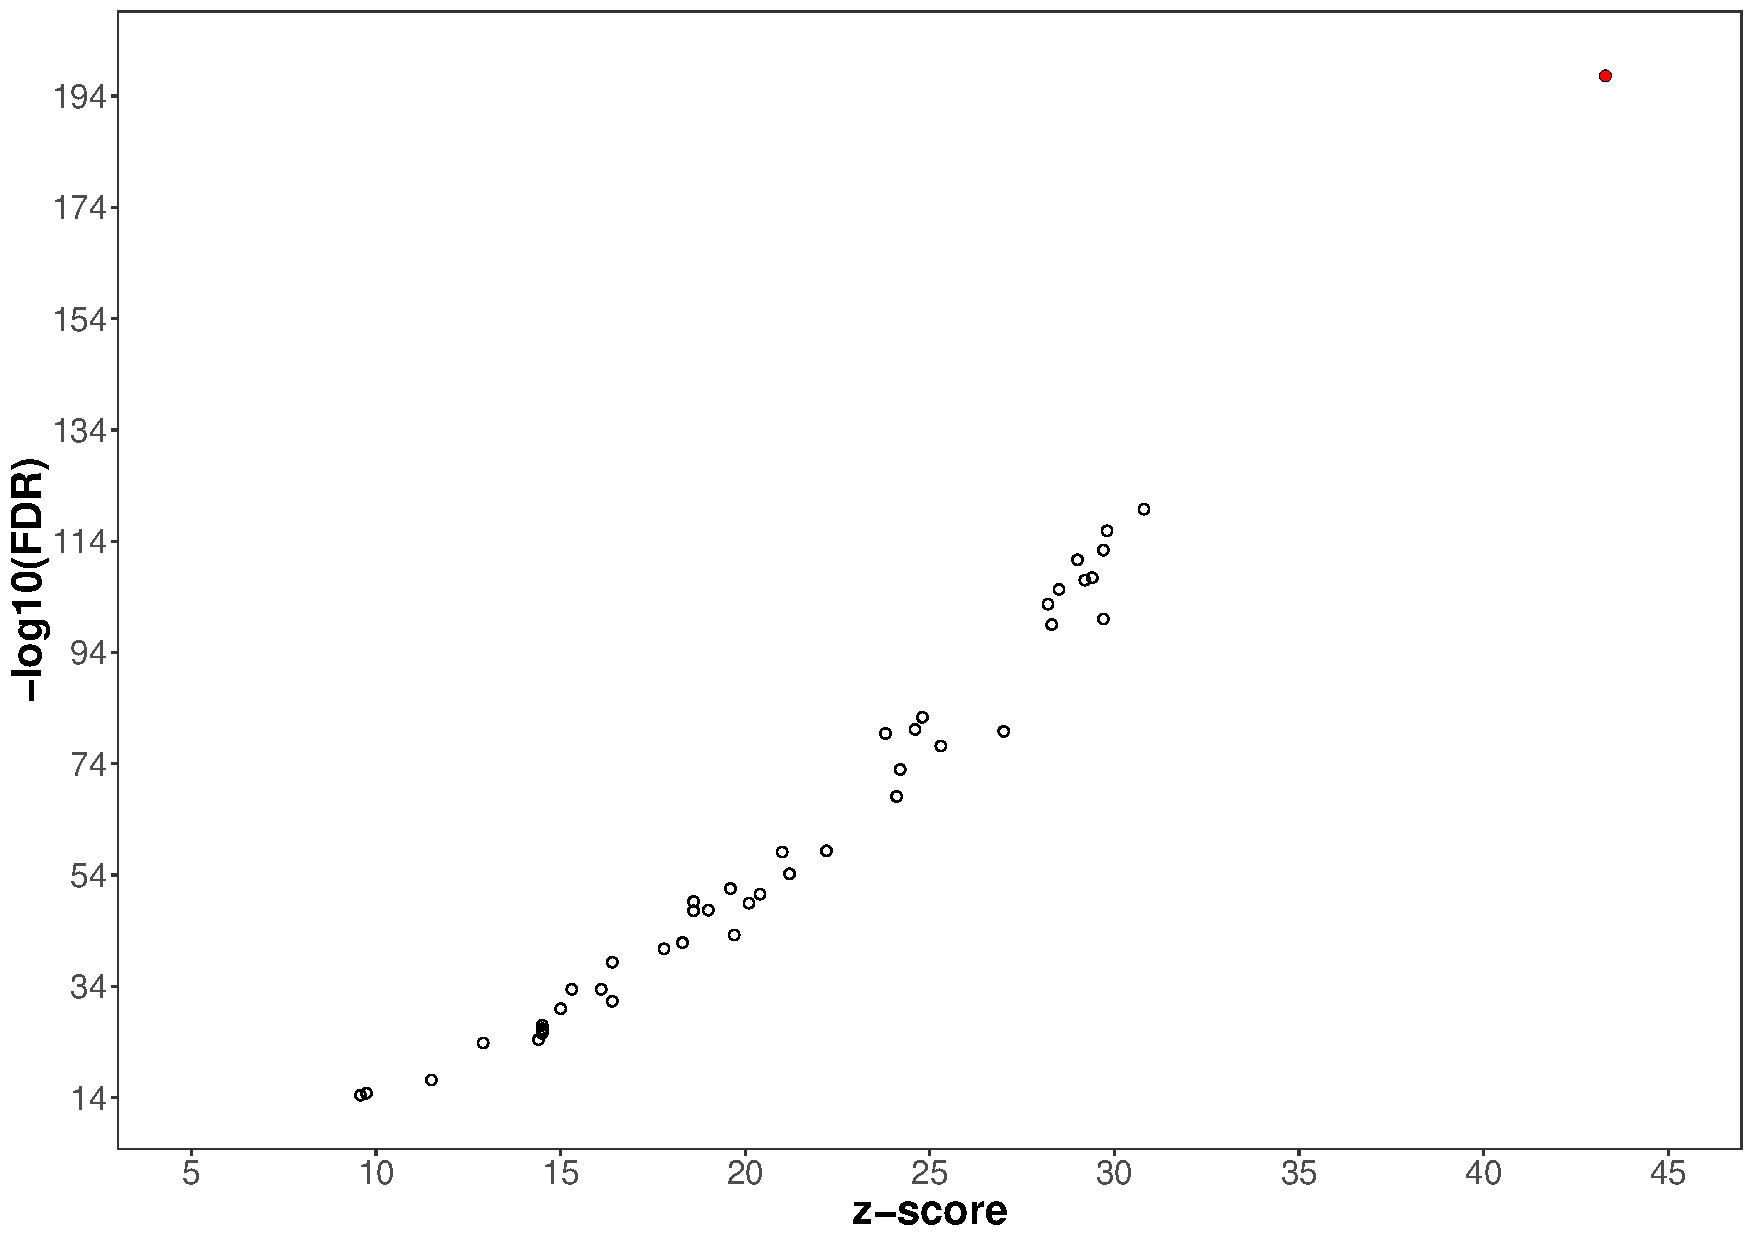
\includegraphics[width=\textwidth]{./Results3/pdfs/ATAC_PSA_all_GTeX_eQTL_enrichment_dotplot}
\caption{}
\end{subfigure}
~
\begin{subfigure}[b]{0.7\textwidth} 
%the [b] prevents offset in subcaptions
\centering
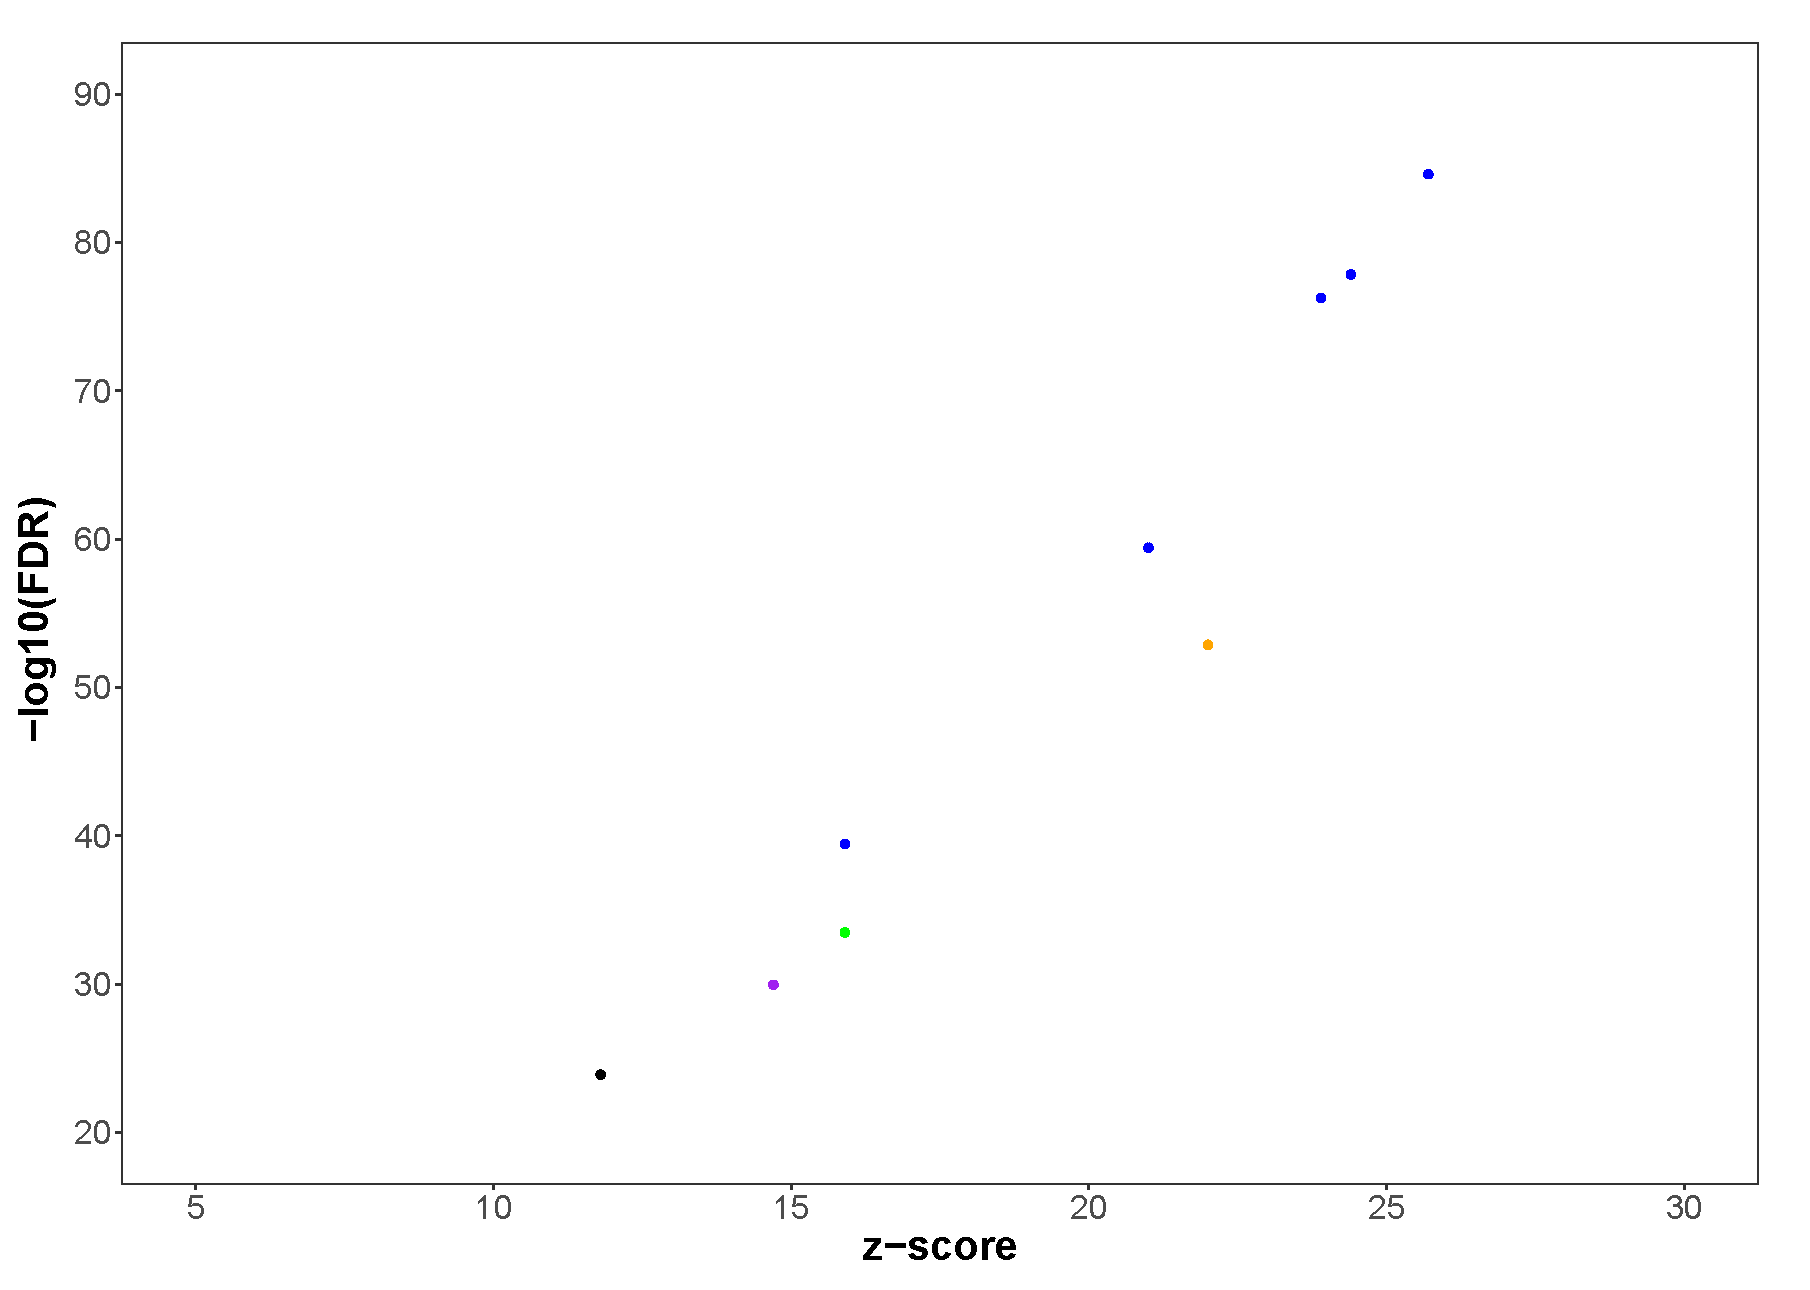
\includegraphics[width=\textwidth]{./Results3/pdfs/ATAC_PSA_all_Jknight_eQTL_enrichment_dotplot}
\caption{}
\end{subfigure}
\caption[Enrichment of eQTLs publicly available data in the combined cell type and tissue chromatin accessibility master list for the PsA cohort.]{\textbf{Enrichment of eQTLs publicly available data in the combined cell type and tissue chromatin accessibility master list for the PsA cohort.} The dot plots showed the z-score values of the enrichment analysis in the x-axis and the significance (-log$_10$FDR) in the y-axis for a) GTEx eQTL datasets and b) non-GTEx immune-related cell types including CD14$^+$ monocytes (unstimulated, 2 or 24h LPS stimulated and 24h IFN$\gamma$ stimulated) in blue, B-cells in black, total CD4$^+$ in green, total CD8$^+$ in orange and neutrophils in purple.}
\label{figure:PsA_FAST_ATAC_eQTL_enrichment}
\end{figure}





\subsubsection{Differential open chromatin analysis between blood and SF}
Differential chromatin accessibility analysis was performed per cell type using a paired design between SF and PB for each of the four cell types (Table \ref{tab:PSA_DOCs_results}. For each of the cell types a master list containing chromatin accessible regions in at leats 30\% of the samples ($\sim$2 samples), regardless the tissue. In all for analysis an 80\% cut-off for background noise was applied to the count matrix, as previously explained in Chapter 3. Only differentially open regions (DORs) identified with DESeq2 and also shared with quantile normalisation limma voom analysis where considered downstream. The CD14$^+$ monocytes and NK showed a greater proportion of DORs (23.3 and 8.9\%, respectively) compared to mCD4$^+$ and mCD8$^+$ T cells. In CD14$^+$ monocytes a significantly greater number of DORs more accessible  in SF (3,779 DORs) were found compared to PB (1,506 DORs). Conversely, the number of open DORs in Sf and PB were evenly distributed between in the other three cell types.


\begin{table}[htbp]
%\setlength{\tabcolsep}{20pt} only to stretch the columns if you want
%\renewcommand{\arraystretch}{1.5}
\centering
\begin{tabular}{@{} c c c c c}
\toprule
\textbf{Cell type}  & \textbf{Total DORs} &  \textbf{Proportion  &\textbf{DORs open} & \textbf{DORs open } \\
                    &                     &  \textbf{DORs (\%)}  &\textbf{in SF}     & \textbf{in PB} \\
\midrule
\midrule
CD14$^+$ & 5,285 & 23.3 & 3,779 & 1,506 \\
CD4$^+$ & 1,329 & 4.3 & 621 & 708 \\
CD8$^+$ & 1,570 & 4.5 & 807 & 763 \\
NK      & 2,314 & 8.9 & 1,223 & 1,091 \\
\bottomrule
\end{tabular}
\medskip %gap
\caption[Summary results of the chromatin accessibility analysis between SF and PB in PsA samples]{\textbf{Summary results of the chromatin accessibility analysis between SF and PB in PsA samples.}}
\label{tab:PSA_DOCs_results}
\end{table}

Permutation analysis using the ten unique possible combinations demonstrated that greater number of DORs than expected by chance were obtained in the differential analysis (Figure \ref{figure:PsA_perm_analysis}). This reinforced the fact that the identified changes in chromatin accessibility are driven by true differences between SF and PB in all the analysed cell types and therefore are specific.
  
When performing genomic annotation of the DORs in each of the cell types, intronic and intergenic regions consistently represented 80\% or more of all regions with differential accessibility (Figure \ref{figure:PsA_FAST_ATAC_DOCS_annotation} a). Universal promoter regions represented the third genomic feature with approximately between 5 to 15\% of the DORs annotation. In addition to this, the fifteen cell type-specific chromatin states from the Epigenome Roadmap segmentation maps were also used for annotation (Figure \ref{figure:PsA_FAST_ATAC_DOCS_annotation} b). For all four cell types DORs, between 44.96 and 72.11\% were annotated as weak enhancers, which represented the most prominent category and the most significantly enriched (data not shown). This was consistent with the predominance of introns and intergenic regions, as those are the preferred location for enhancer elements. Although modest percentages of heterochromatin and repetitive regions were observed, enrichment was not significant for these two chromatin states in any of the four cell types (data not shown).

\bigskip
\begin{figure}[H]
\centering
\begin{subfigure}[b]{0.7\textwidth}
\centering 
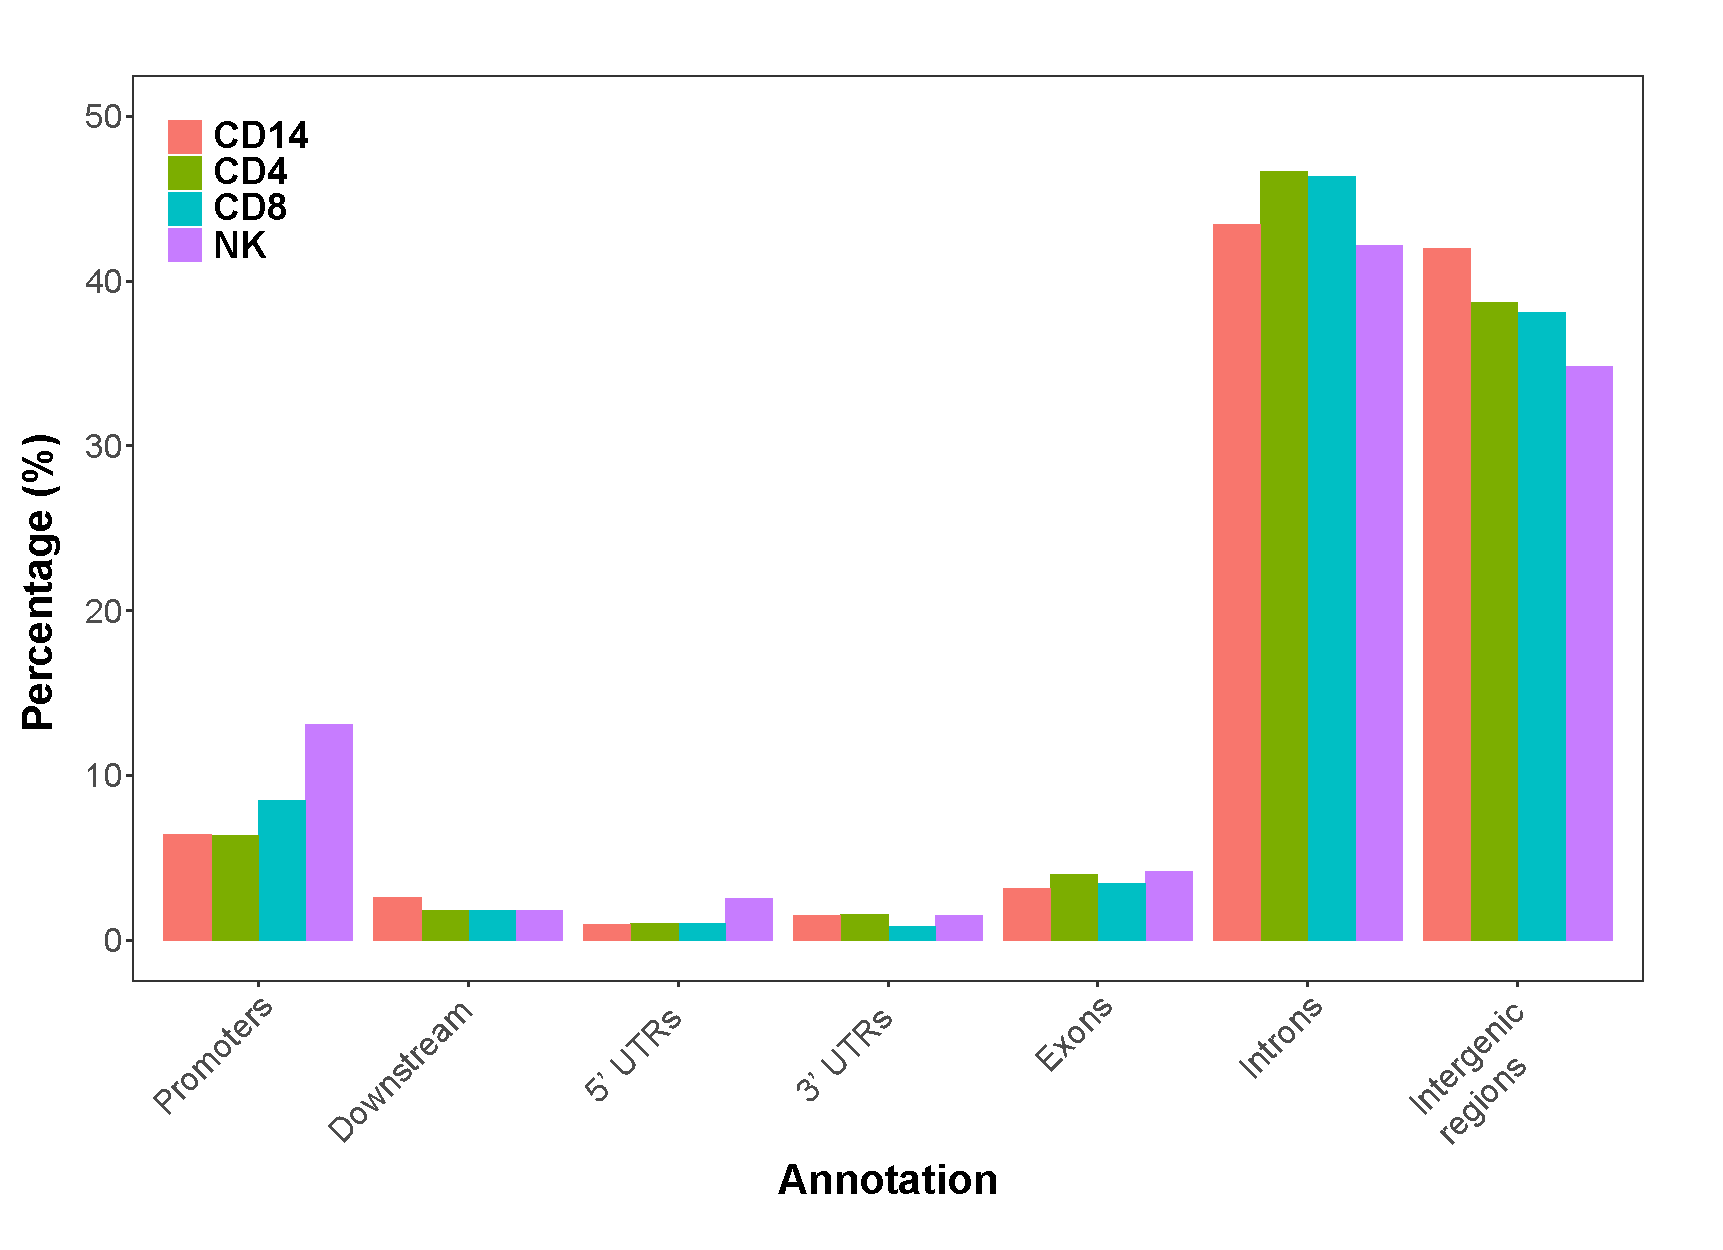
\includegraphics[width=\textwidth]{./Results3/pdfs/ATAC_PSA__DOCS_per_cell_type_general_annotation}
\caption{}
\end{subfigure}
~
\begin{subfigure}[b]{0.7\textwidth} 
%the [b] prevents offset in subcaptions
\centering
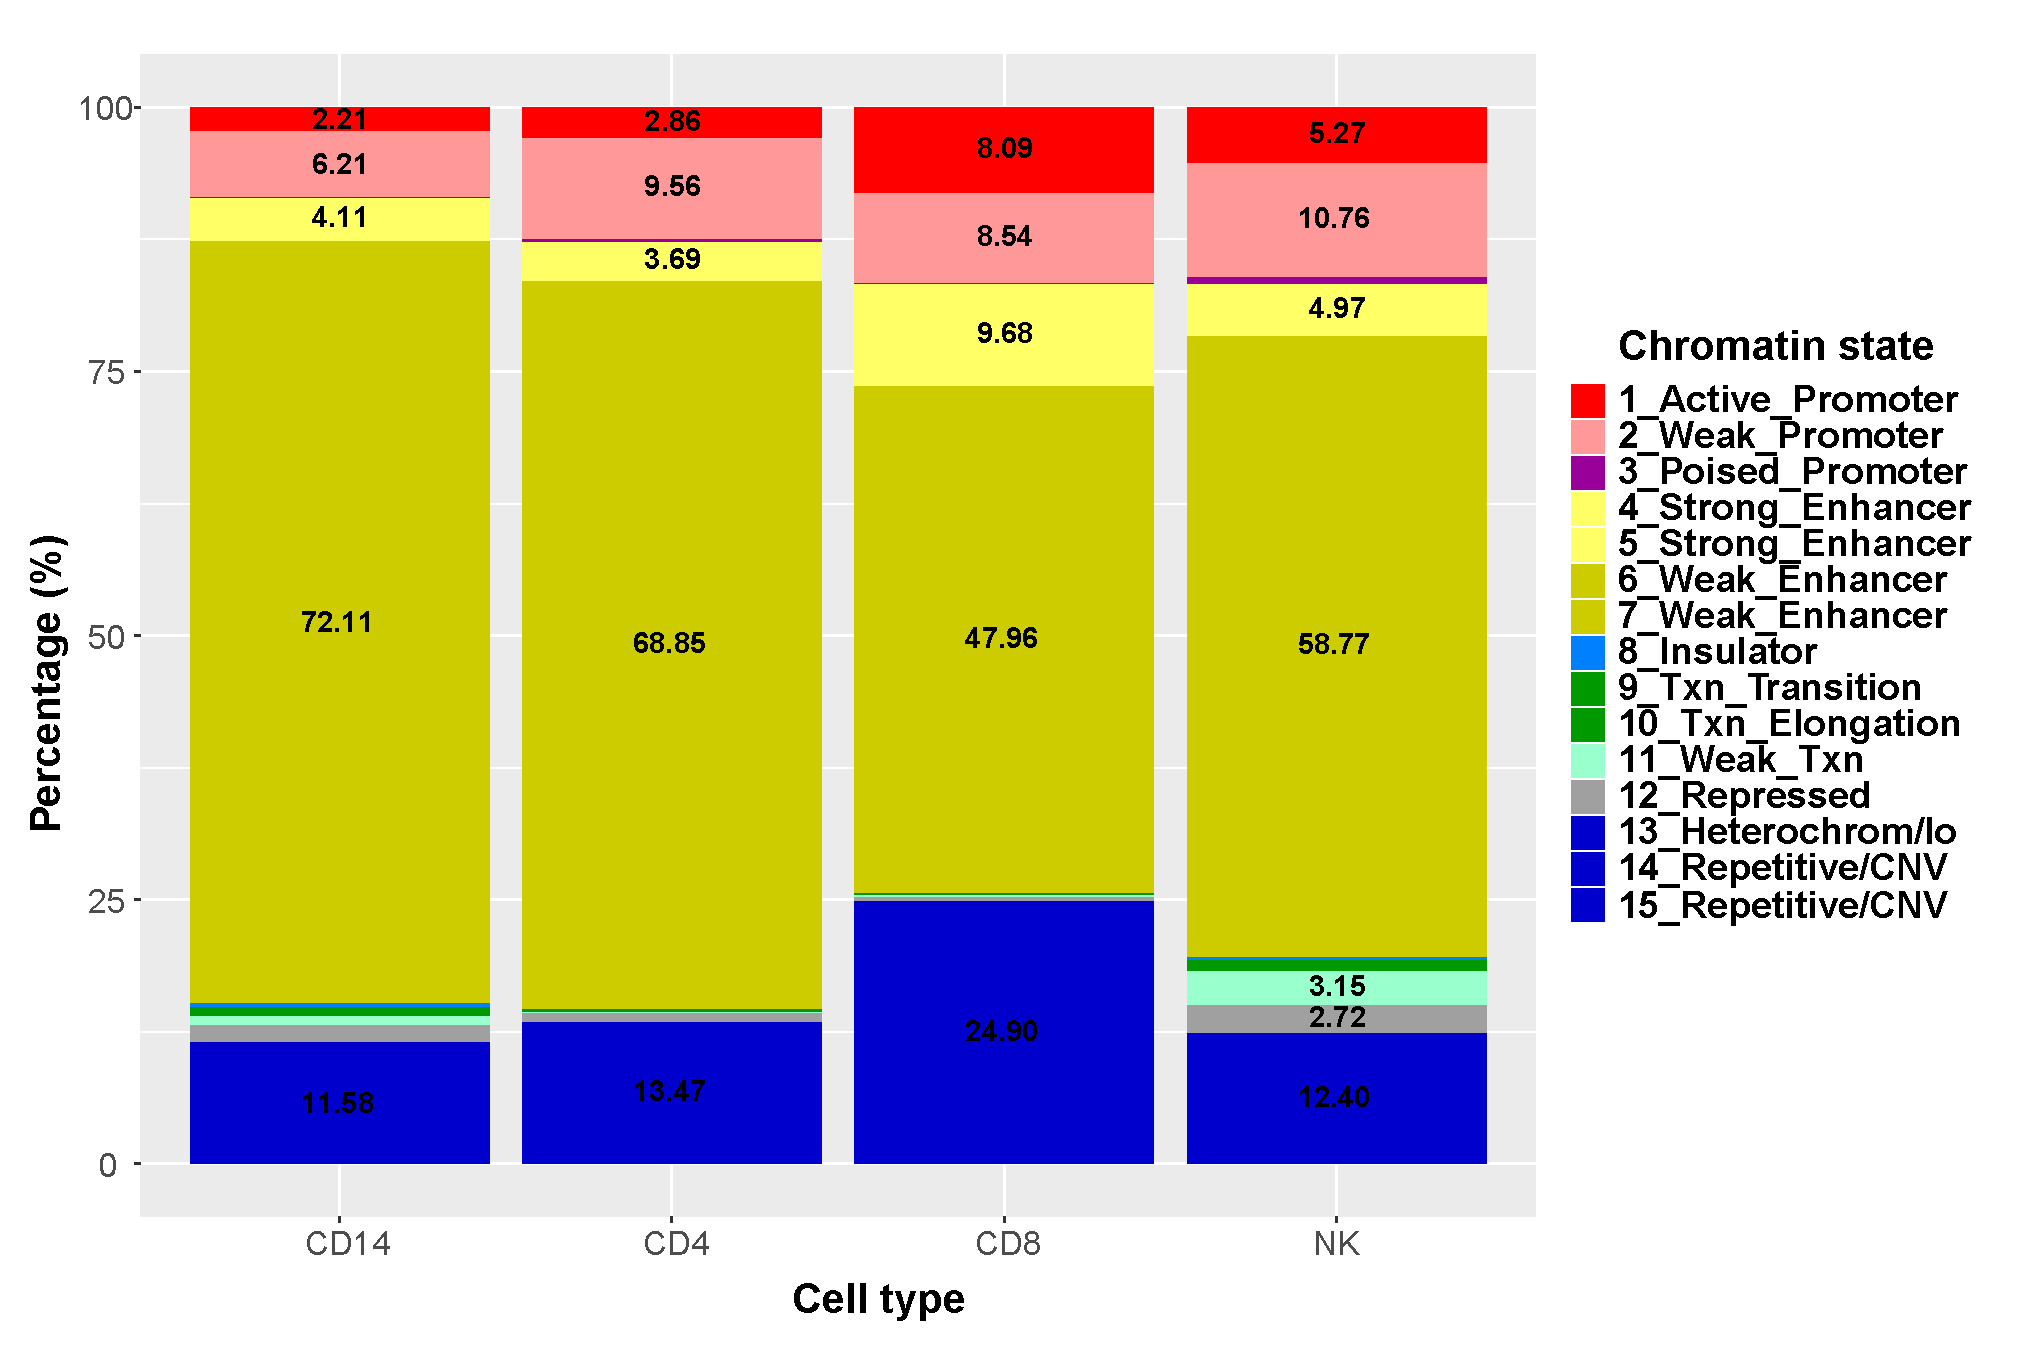
\includegraphics[width=\textwidth]{./Results3/pdfs/ATAC_PSA_DOCS_chromatin_states_stacked_barplot}
\caption{}
\end{subfigure}
\caption[Annotation with genomic regions and chromatin states of the PsA DOCs from the four cell types differential analysis.]{\textbf{Annotation with genomic regions and chromatin states of the PsA DOCs from the four cell types differential analysis.} xxxx}
\label{figure:PsA_FAST_ATAC_DOCS_annotation}
\end{figure}


%Try to overlap the enhancer FANTOM data to id those regions whith evidence of eRNA expression
The functional relevance of the differential chromatin accessibility in terms of regulation of gene expression was further investigated by integration of the eRNA data from the FANTOM5 project. Statistically significant enrichment for robust and permissive enhancers was found for the DORs identified in the four cell types (Figure \ref{figure:PSA_FANTOM}). Robust enhancers are those for which transcription was significantly detected at the genome-wide level in at least one primary cell type or tissue, whereas the permissive set included also those not passing the filtering criteria \parencite{Andersson2014}. Moreover, DORs from all four cell types also presented significant enrichment for the corresponding cell type eRNA set amongst the top two most enriched. The proportion of DORs overlapping the appropriate cell type set of expressed eRNAs ranged between 19.8\% (83 open in SF and 160 open in PB)in NK and 31.8\% (83 open in SF and 160 open in PB) in CD4$^+$.


\begin{figure}[htbp]
\centering
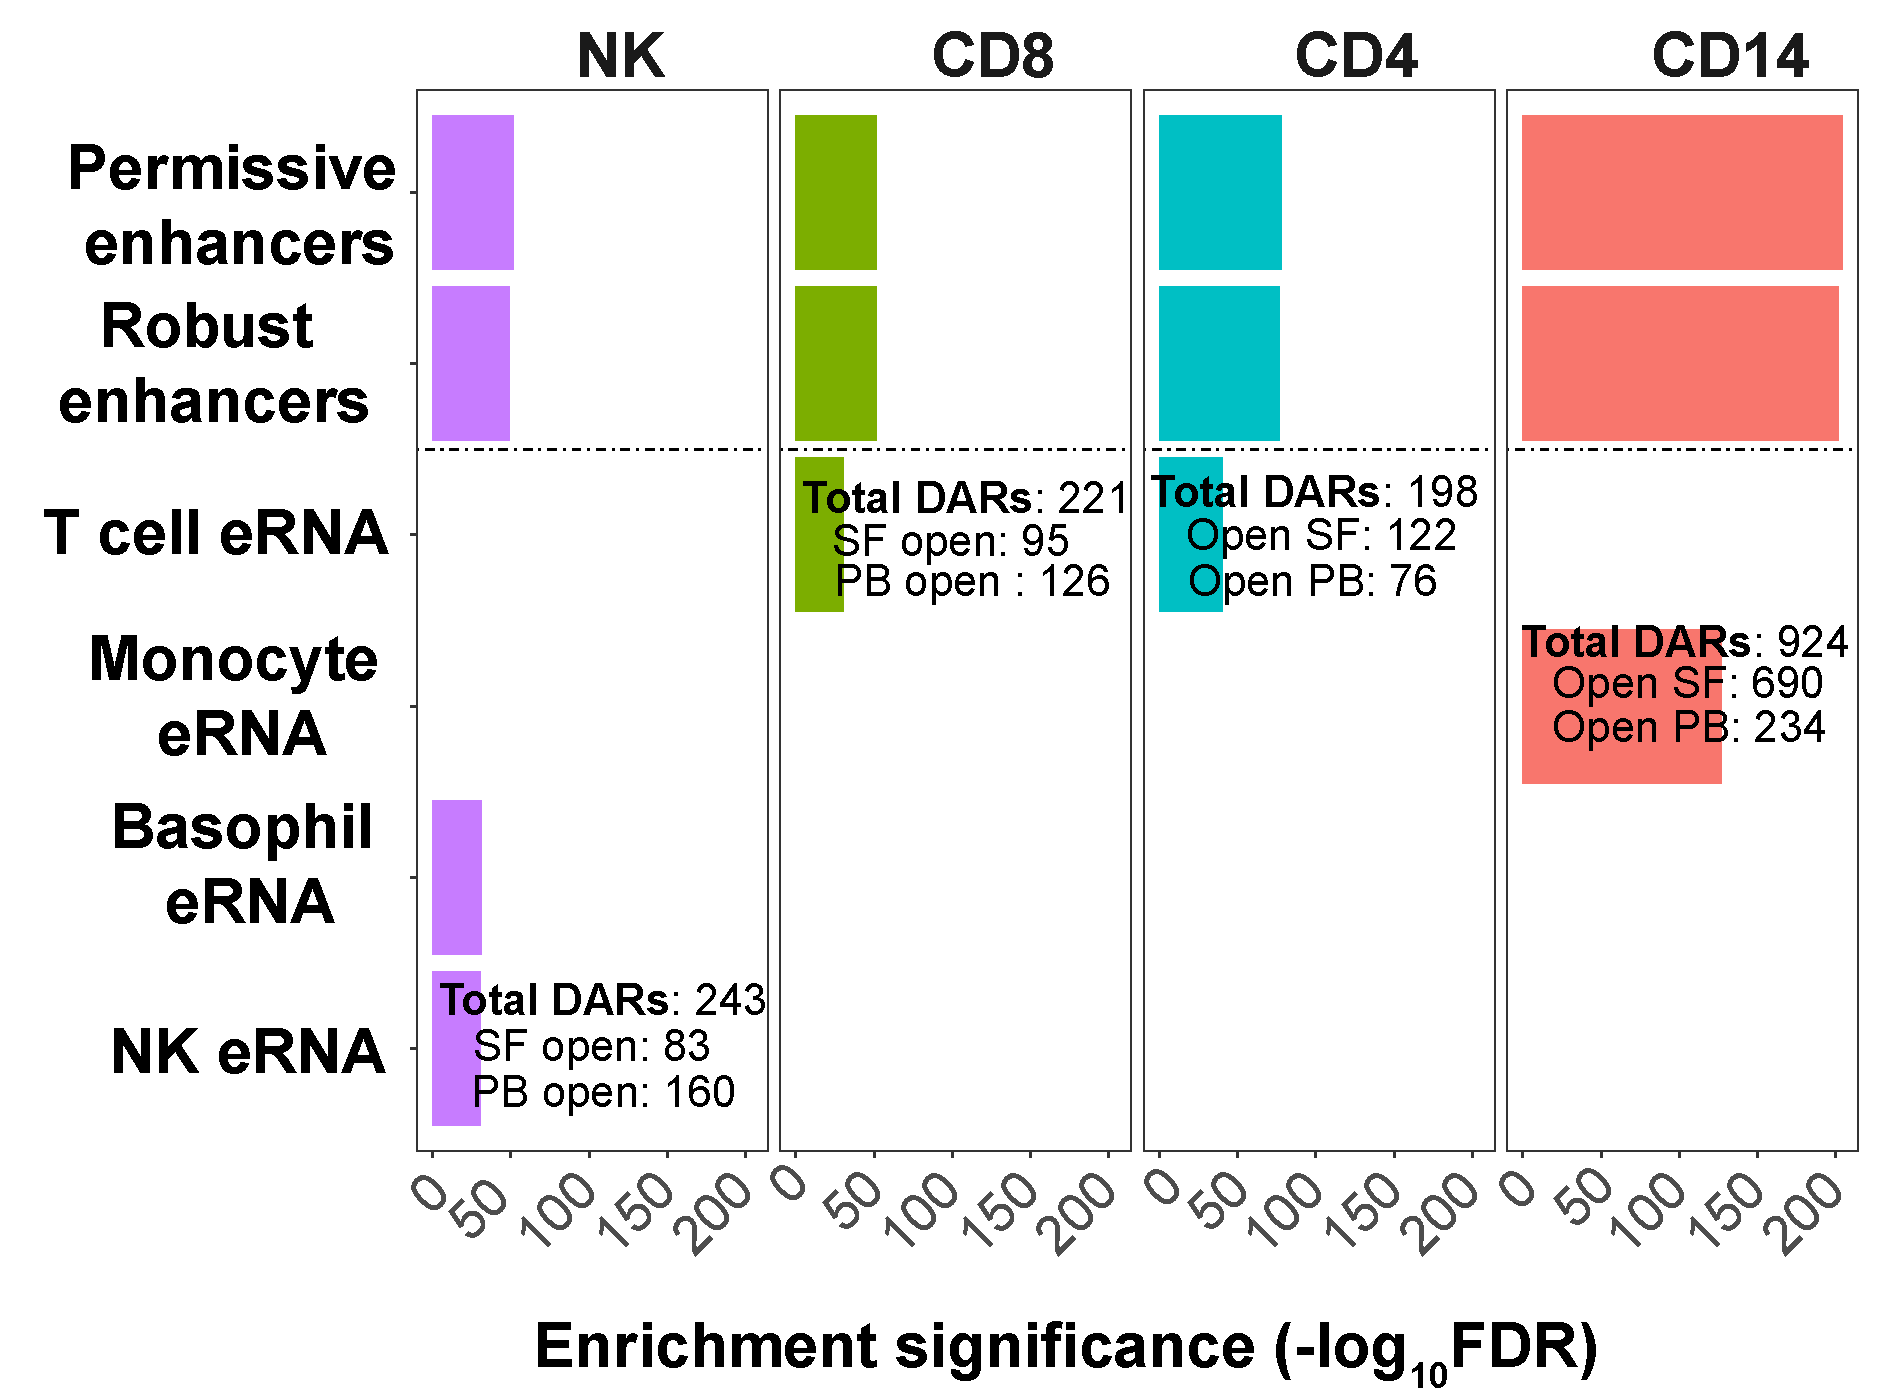
\includegraphics[width=0.8\textwidth]{./Results3/pdfs/ATAC_PsA_FANTOM_enhancer_enrichment_all_cell_types}
\caption[Enrichment of PsA DOCs for the FANTOM5 eRNA dataset]{\textbf{Enrichment of PsA DOCs for the FANTOM5 eRNA dataset.}  }
\label{fig:PSA_FANTOM}
\end{figure}

From the differential analysis between SF and PB in all four cell types, a number of DORs were overlapping a gene body (Table \ref{tab:PSA_DOCs_gene_body}). Interestingly, the majority were located within introns instead of untranslated regions (UTRs) and have also been annotated as weak or strong enhancers according to the cell type specific chromatin segmentation map. 

%Similarly, more accessible chromatin in SF compared to PB was identified in five regions of the \textit{IL15} gene, annotated as promoter and enhancers in CD14$^+$ monocytes. 
% Check differences at both gene locations were CD14$^+$ cell type specific is this region HiC annotated with the gene? and maybe include example overlapping eRNA
%e.g LMNA4 which is CD14 cell specific and more expressed in SF in Dolcino paper. Maybe use it later

\begin{table}[htbp]
%\setlength{\tabcolsep}{20pt} only to stretch the columns if you want
%\renewcommand{\arraystretch}{1.5}
\centering
\begin{tabular}{@{} c c c c c}
\toprule
\textbf{Cell type} & \textbf{DORs in gene body} &  \textbf{Gene with $>$ one DOR} &\textbf{Enhancers} & \textbf{Introns} \\
\midrule
\midrule
CD14$^+$ & 2,357 & 744 & 1,775 & 1,920 \\
CD4$^+$ & 700 & 99 & 504 & 577 \\
CD8$^+$ & 831 & 118 & 503 & 666 \\
NK   & 1,246 & 235 & 782 & 937 \\   
\bottomrule
\end{tabular}
\medskip %gap
\caption[Annotation of gene body DORs in four cell types from PsA samples.]{\textbf{Annotation of gene body DORs in four cell types from PsA samples.}}
\label{tab:PSA_DOCs_gene_body}
\end{table}

As an example, a more accessible PB DOR located in an intron of the \textit{VAV3} gene and significantly expressed as eRNA was identified in NK (Figure \ref{figure:PsA_FAST_ATAC_gene_boy_DOCS_CD14_NK} a). Additionally, for all four cell types, a number of gene entities contained more than one DOR, showing the same direction of chromatin accessibility between SF and PB. For example, in CD14$^+$ two DORs located at the 5' and 3'UTRs for \tetxit{IL7R} gene where found to be more accessible in SF compared to PB (Figure \ref{figure:PsA_FAST_ATAC_gene_boy_DOCS_CD14_NK} b). 

\bigskip
\begin{figure}[H]
\centering
\begin{subfigure}[b]{0.70\textwidth}
\centering 
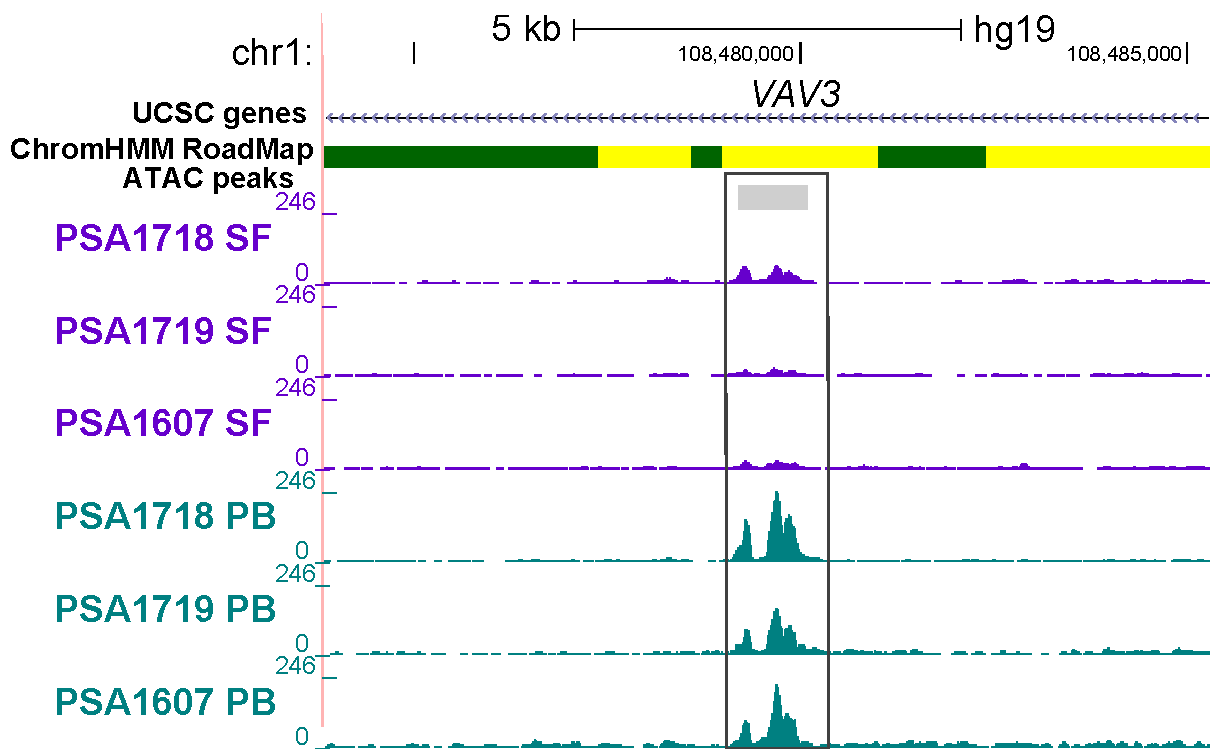
\includegraphics[width=\textwidth]{./Results3/pdfs/ATAC_PSA_NK_VAV3}
\caption{}
\end{subfigure}
~
\begin{subfigure}[b]{0.70\textwidth} 
%the [b] prevents offset in subcaptions
\centering
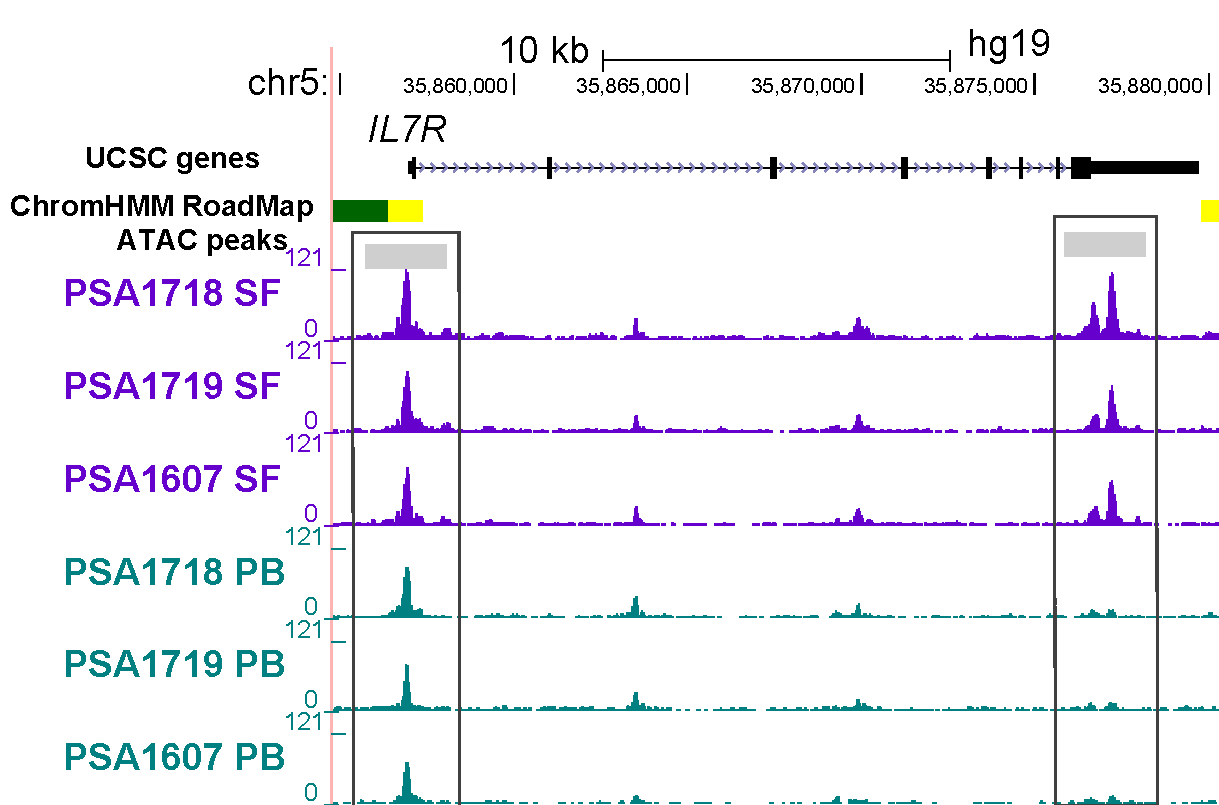
\includegraphics[width=\textwidth]{./Results3/pdfs/ATAC_PSA_CD14_IL7R}
\caption{}
\end{subfigure}
\caption[Differentially accessible regions located within gene bodies in CD14$^+$ monocytes and NK cells from PsA patients.]{\textbf{Differentially accessible regions located within gene bodies in CD14$^+$ monocytes and NK cells from PsA patients.} xxxx}
\label{figure:PsA_FAST_ATAC_gene_boy_DOCS_CD14_NK}
\end{figure}


\subsection{Pathway and TFBS enrichment analysis highlight functional tissue-specific differences in chromatin accessibility}

For each of the four sets of DORs, pathway enrichment analysis was conducted separately for those regions more accessible in SF and PB. Gene annotation of the DORs was performed by physical proximity, as detailed in Chapter \ref{ch:Mat}. Despite commonalities, differences in significant enriched pathways (FDR$<0.01$) were identified within the same cell type between SF and PB (Figure \ref{figure:PSA_ATAC_pathway_analysis_all_DOC}).


\begin{figure}[H]
\centering
\begin{subfigure}[b]{0.45\textwidth}
\centering 
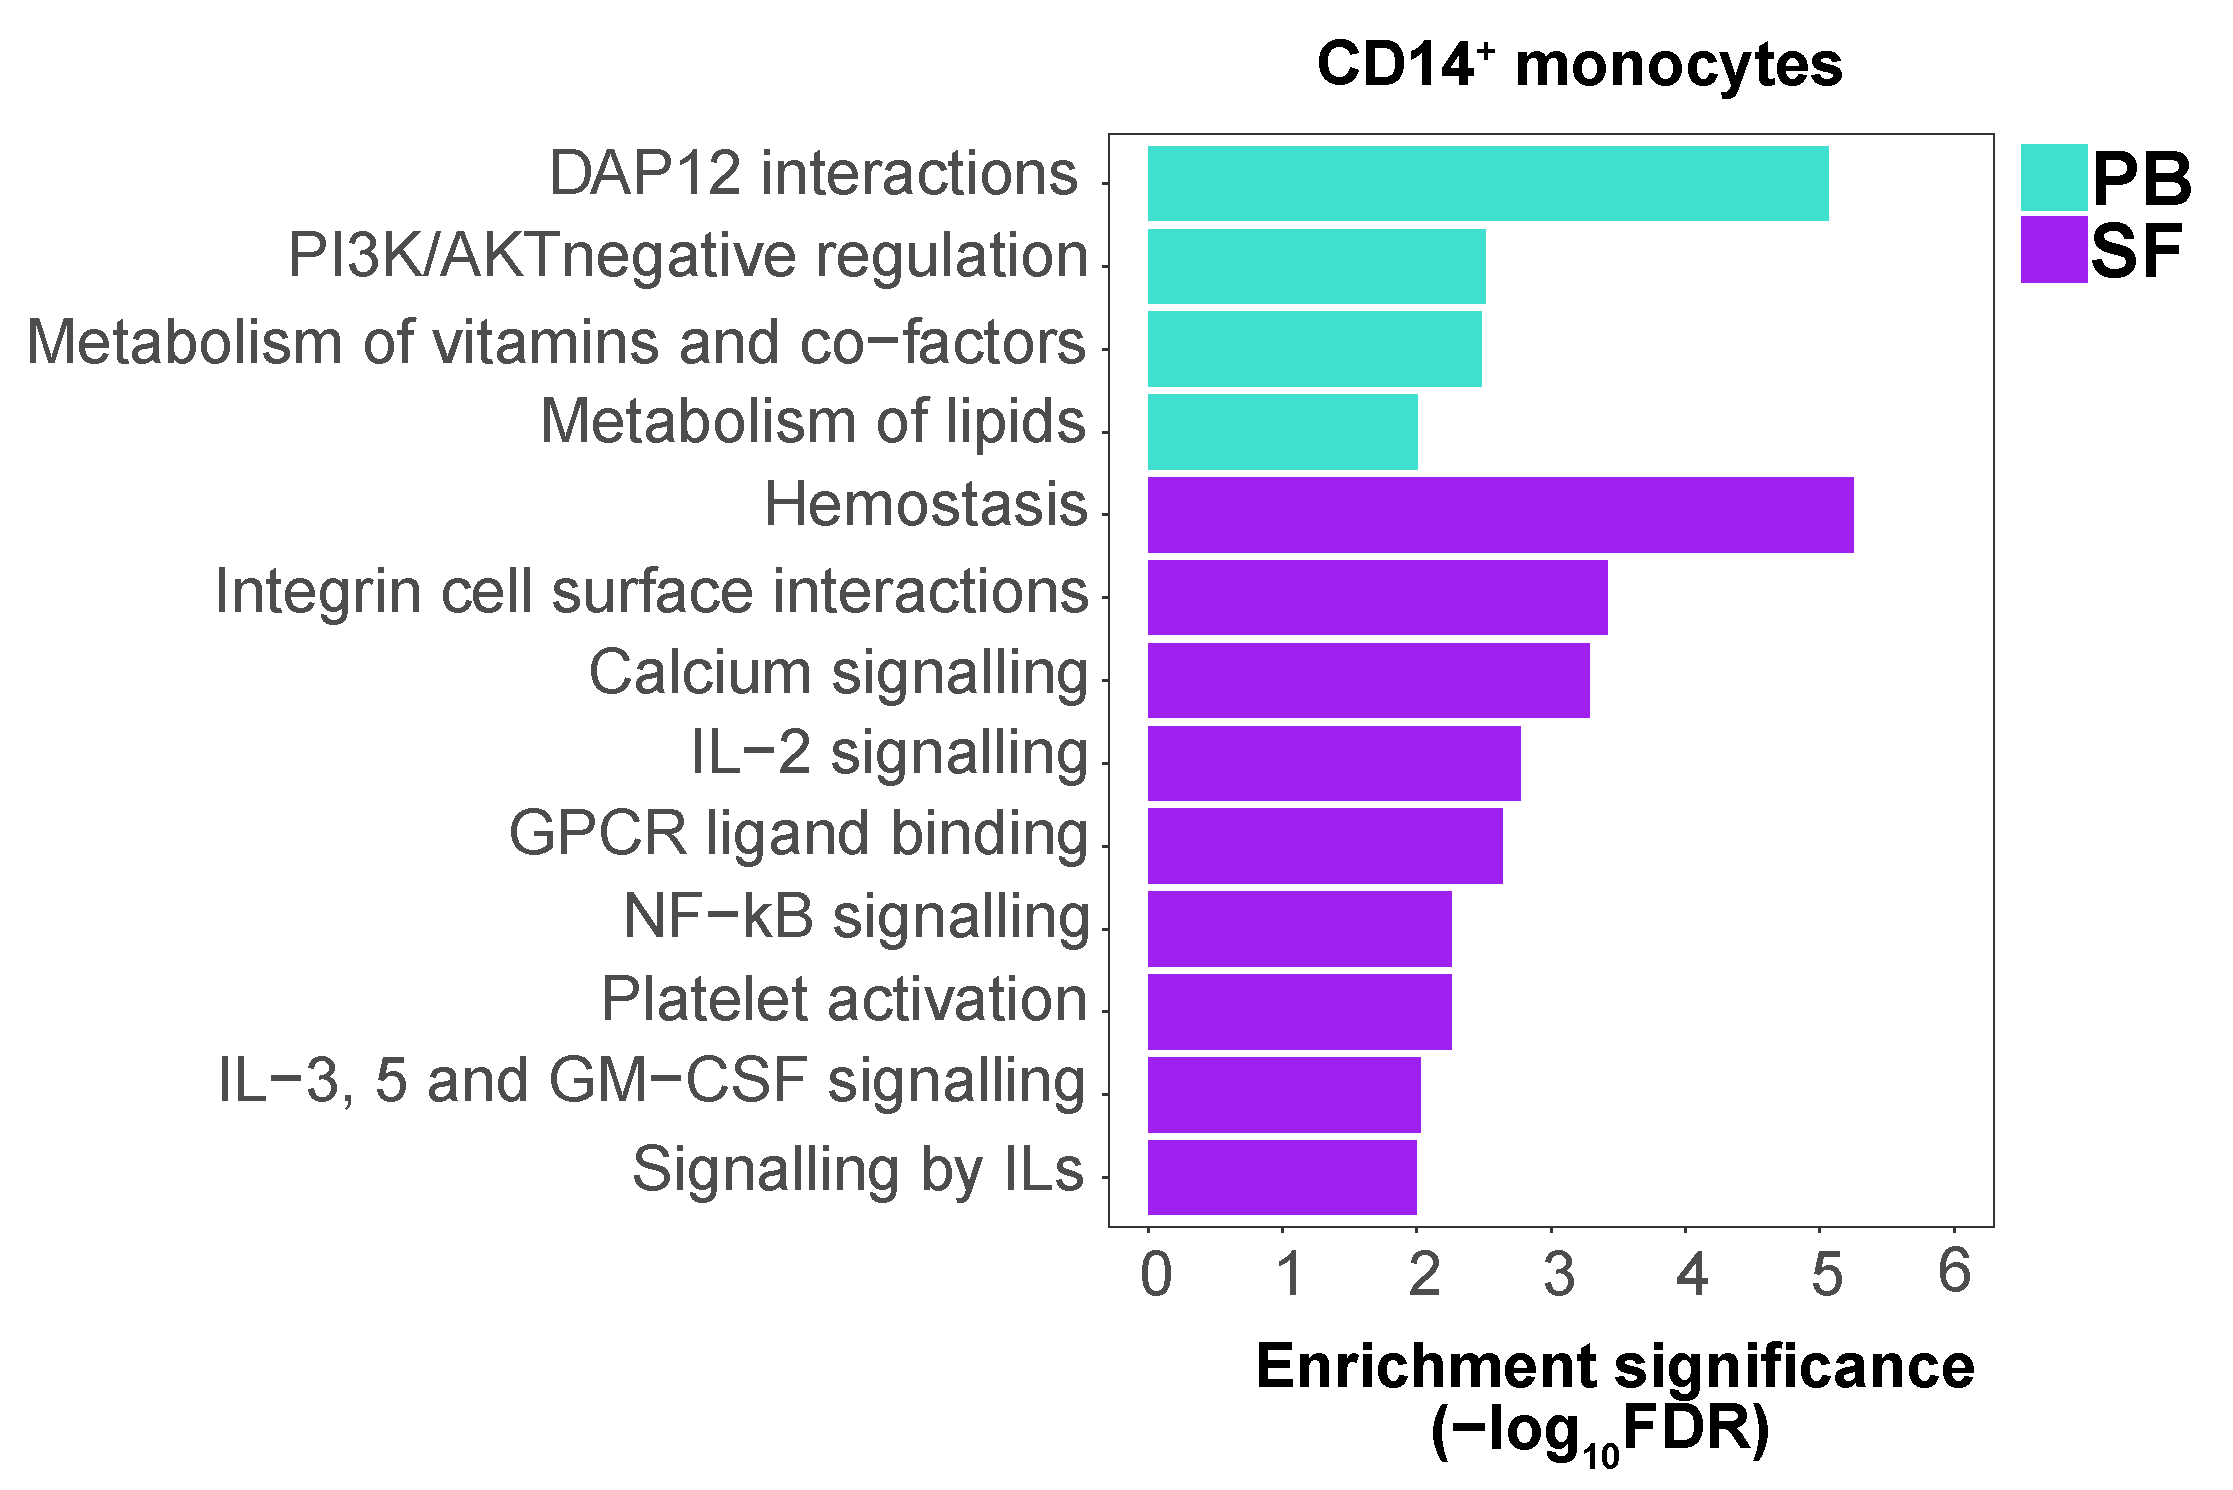
\includegraphics[width=\textwidth]{./Results3/pdfs/ATAC_PSA_CD14_pathways_barplot_all_DOCS_proximity}
\caption{}
\end{subfigure}
~
\begin{subfigure}[b]{0.45\textwidth}
\centering 
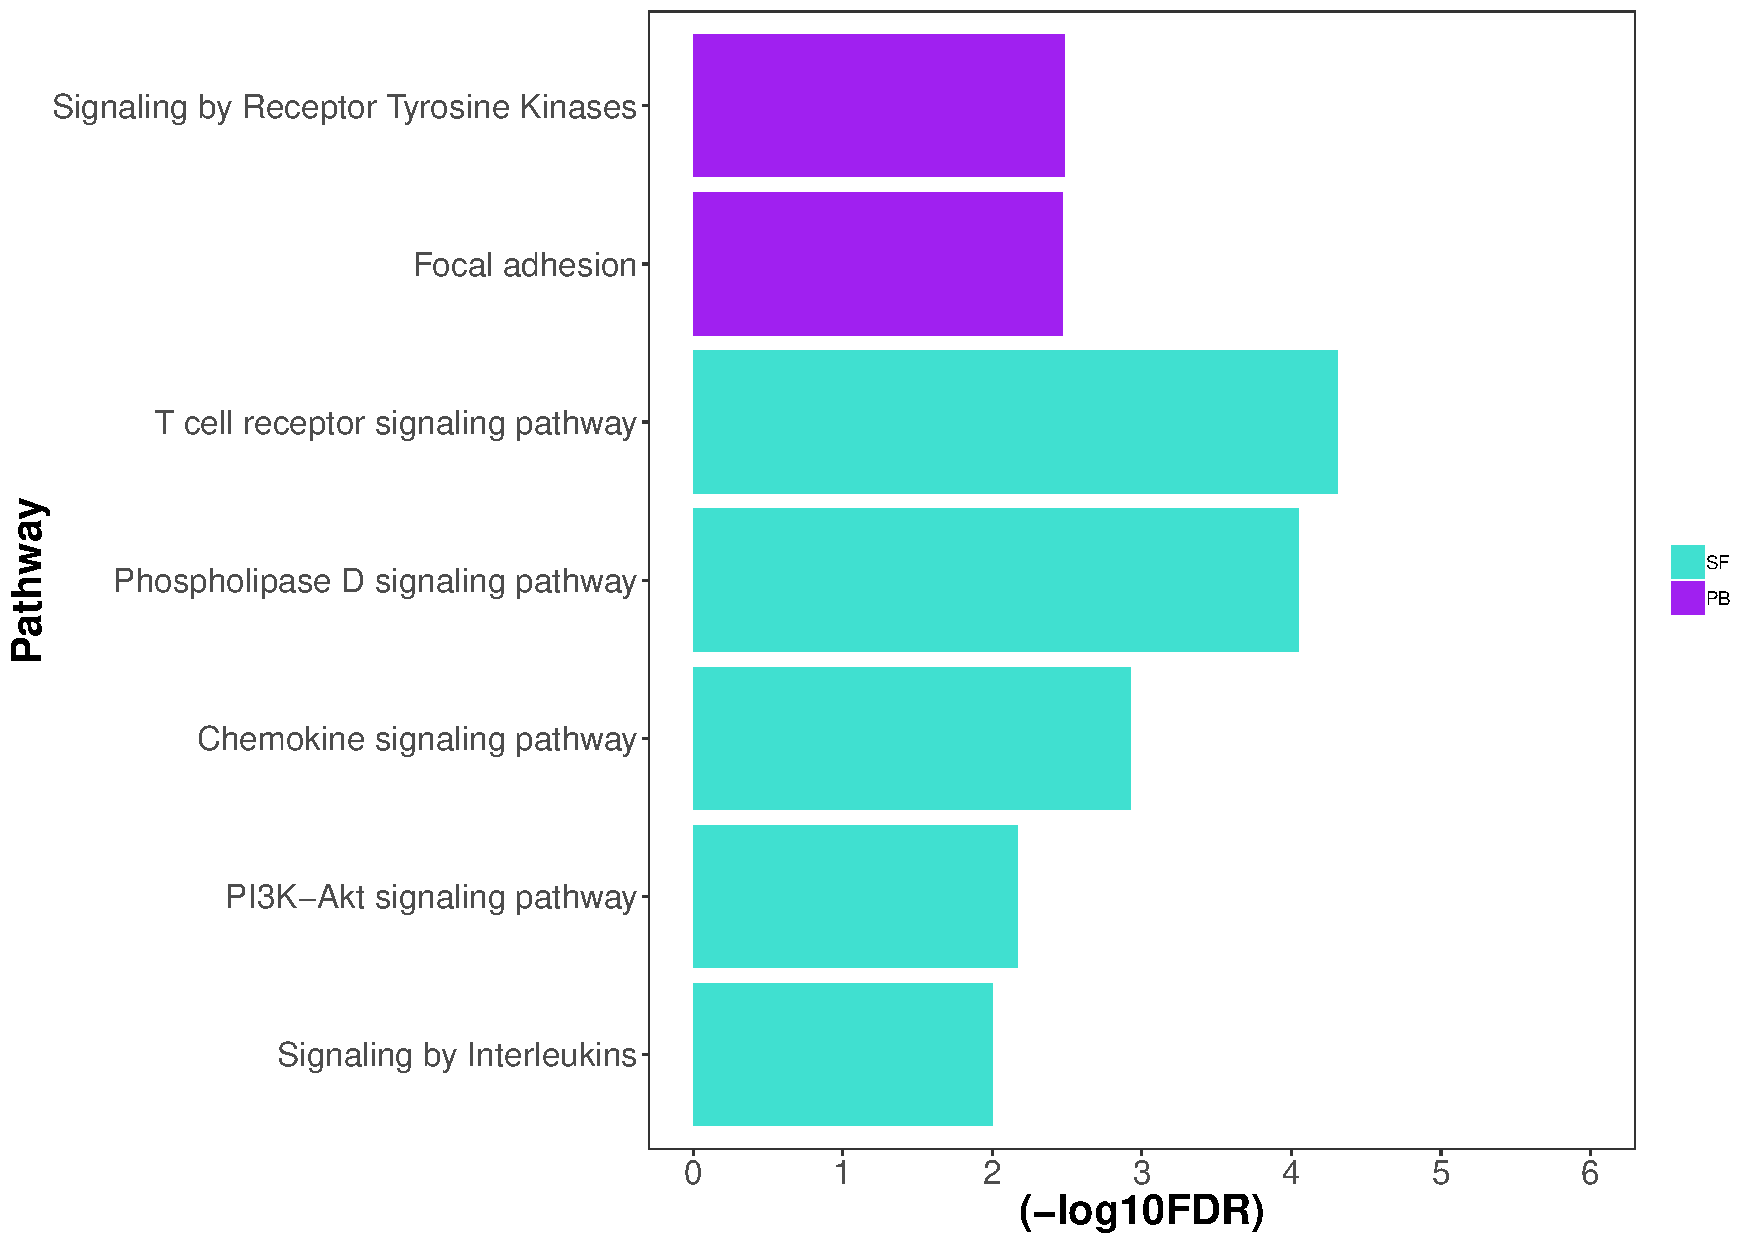
\includegraphics[width=\textwidth]{./Results3/pdfs/ATAC_PSA_CD4_pathways_barplot_all_DOCS_proximity}
\caption{}
\end{subfigure}
~
\begin{subfigure}[b]{0.45\textwidth} 
%the [b] prevents offset in subcaptions
\centering
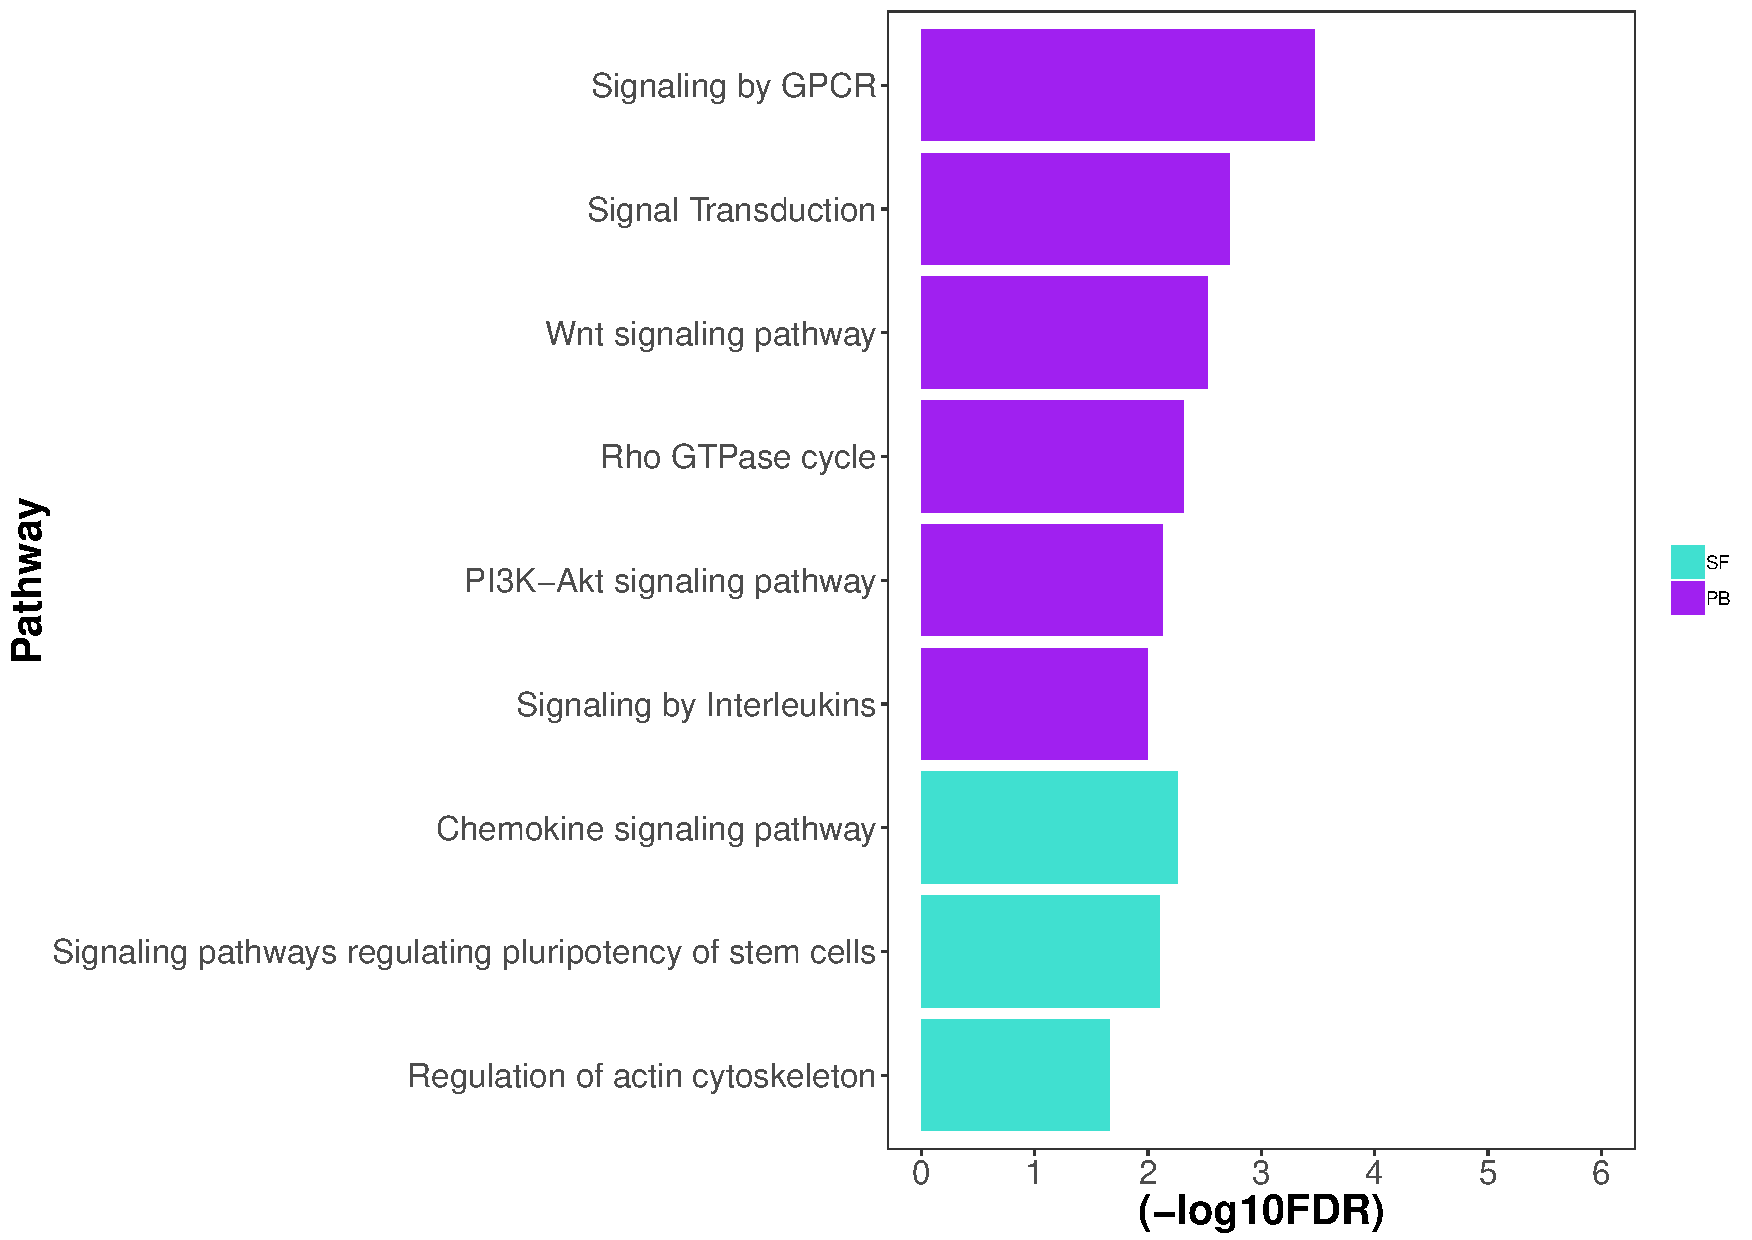
\includegraphics[width=\textwidth]{./Results3/pdfs/ATAC_PSA_CD8_pathways_barplot_all_DOCS_proximity}%
\caption{}
\end{subfigure}
\begin{subfigure}[b]{0.45\textwidth} 
%the [b] prevents offset in subcaptions
\centering
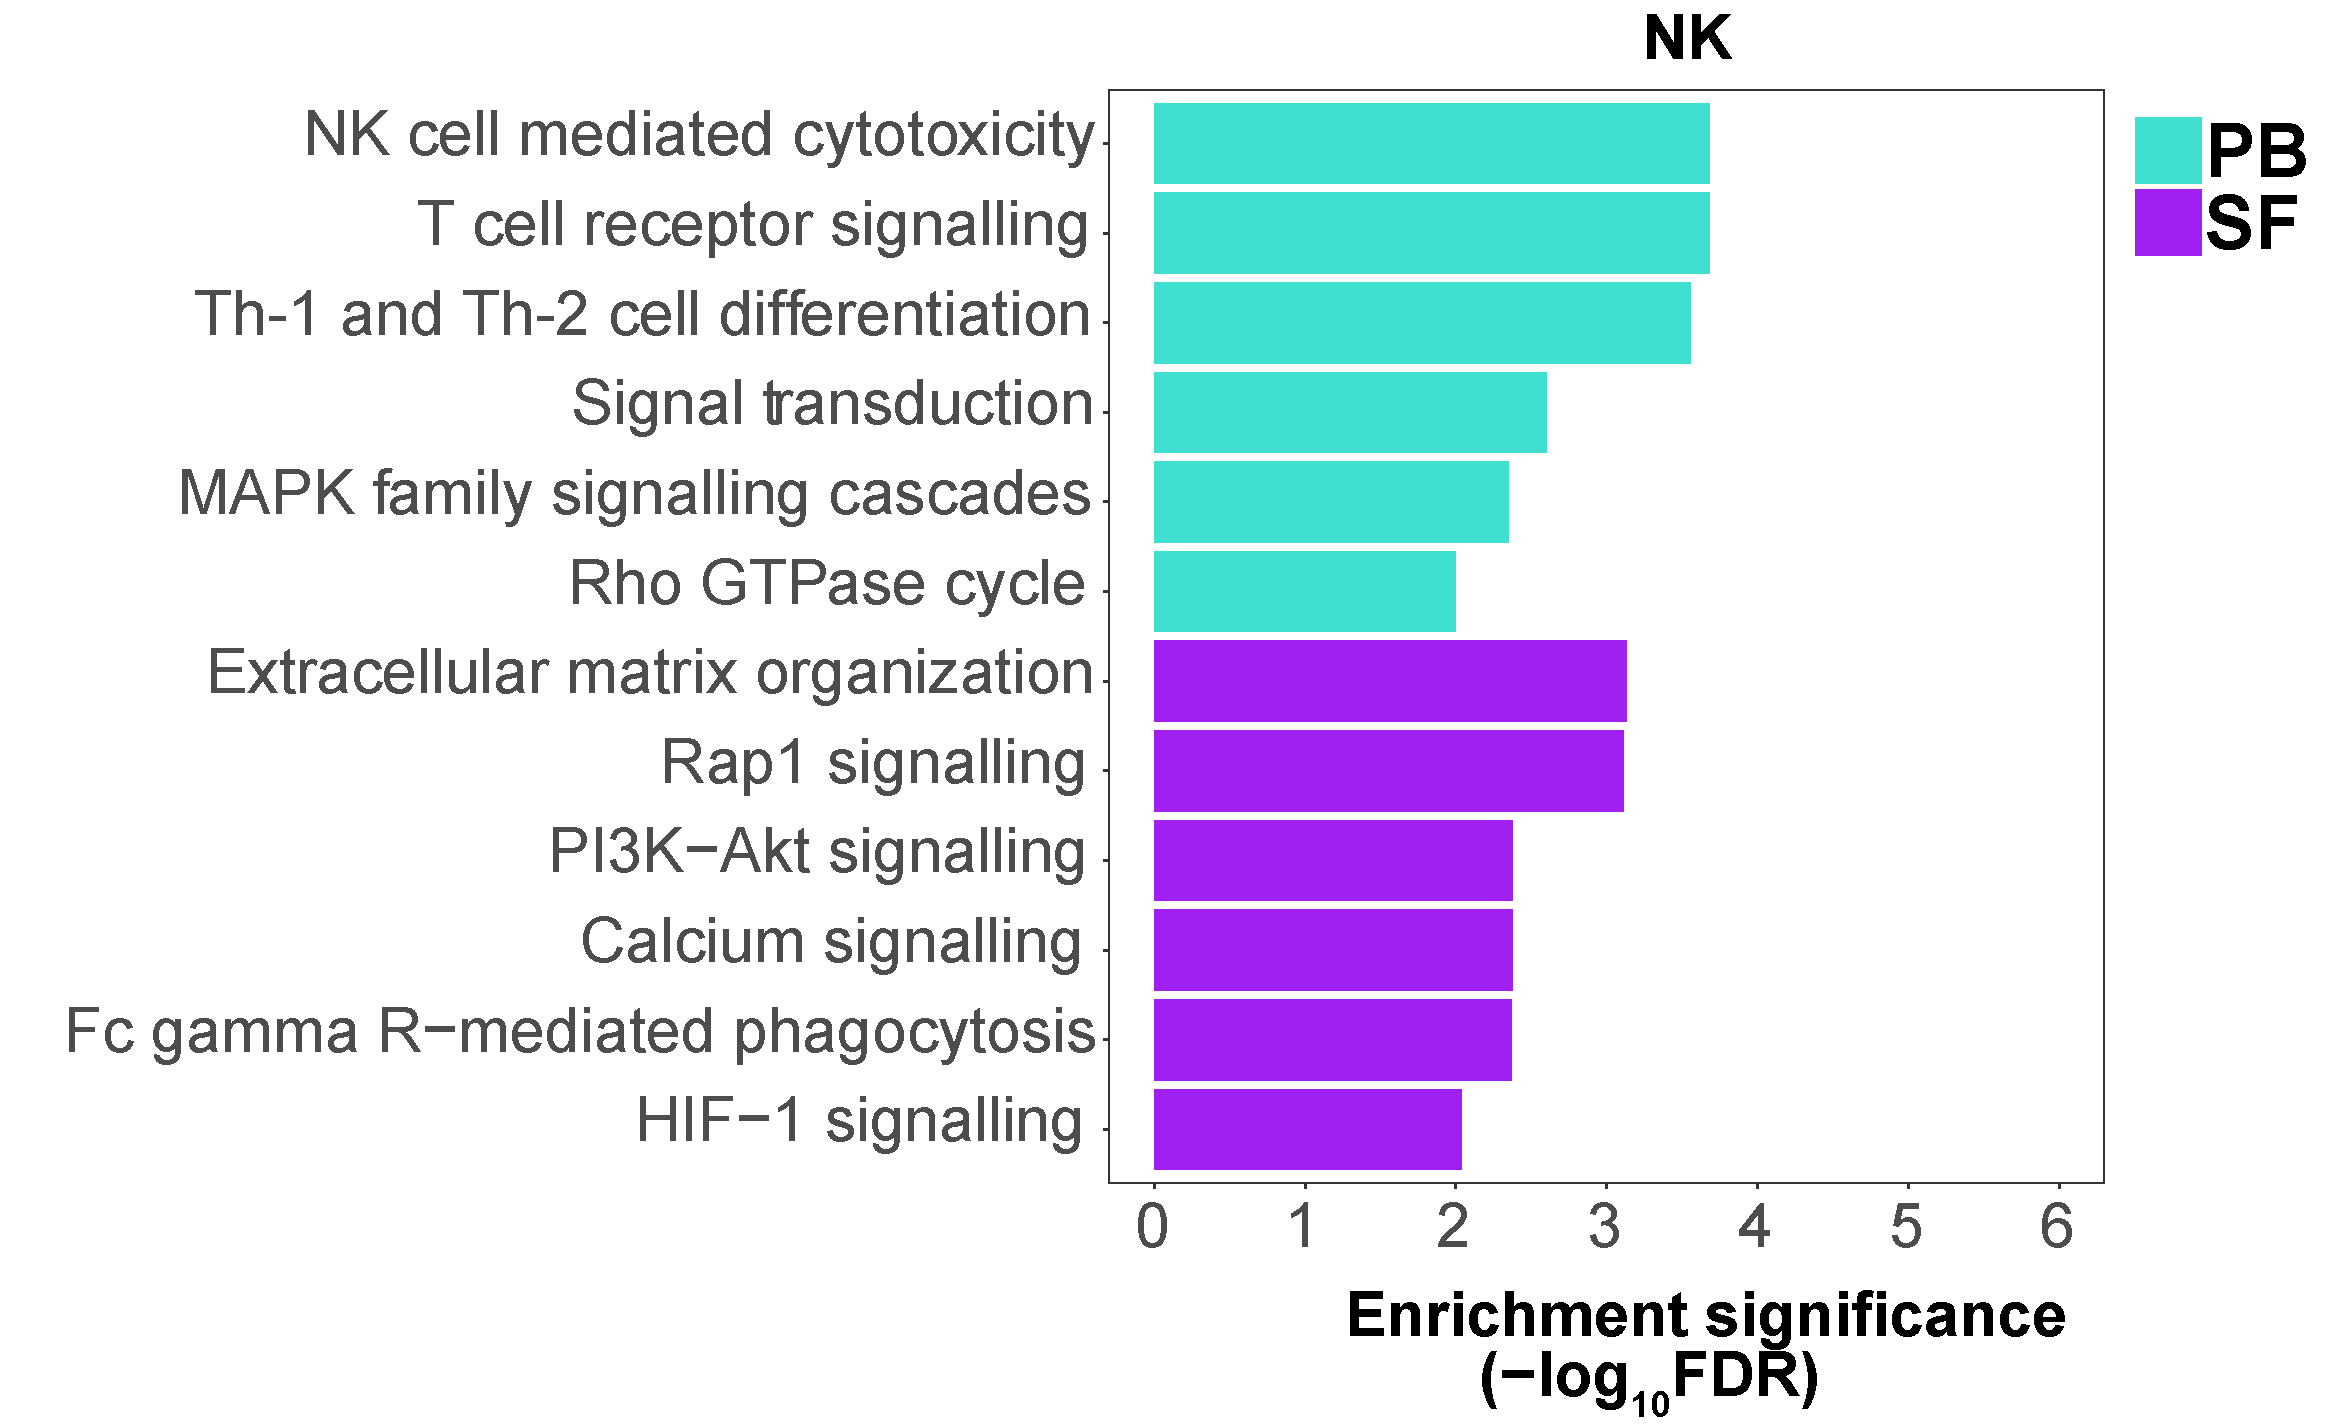
\includegraphics[width=\textwidth]{./Results3/pdfs/ATAC_PSA_NK_pathways_barplot_all_DOCS_proximity}%
\caption{}
\end{subfigure}
\caption[Distinct enriched pathways across SF and PB in CD14$^+$,CD4m$^+$,CD8m$^+$ and NK.]{\textbf{Distinct enriched pathways across SF and PB in CD14$^+$,CD4m$^+$,CD8m$^+$ and NK.} All pathways shown have an FDR $<$0.01. }
\label{figure:PSA_ATAC_pathway_analysis_all_DOC}
\end{figure}




%Decide if table or barplots
%\begin{landscape}
%\begin{center}
%\begin{longtable}[ht]{c c c }
%\caption[Distinct enriched pathways in CD14$^+$, mCD4$^+$, mCD8$^+$ and NK between SF and PB]{\textbf{Distinct enriched pathways in CD14$^+$, mCD4$^+$, mCD8$^+$ and NK between SF and PB.} All pathways shown have an FDR $<$0.01.}
%\\
%\label{table:PSA_ATAC_pathway_analysis_all_DOC} \\
%\toprule
%\textbf{Cell type} & \textbf{SF} & \textbf{PB} \\						
%\midrule
%\midrule
%CD14$^+$ & Hemostasis, Platelet activation, Signaling by VEGF & DAP12 interactions, Metabolism of lipids, \\ 
         %& GPCR ligand binding, IL-2 signaling pathway, & Metabolism of vitamins and co-factors, \\ 
         %& Integrin cell surface interactions,NF-kappa B signaling pathway & Negative regulation of the PI3K/AKT network. \\ 
         %& IL-2 family signaling, IL-3, 5 and GM-CSF signaling. & \\ 
%\midrule
%\textbf{mCD4$^+$} & T cell receptor signaling pathway, Phospholipase D signaling pathway ,& Signaling by Receptor Tyrosine Kinases,\\ 
									%& Chemokine signaling pathway, PI3K-Akt signaling pathway, & Focal adhesion.\\ 
									%& Signaling by interleukins. & \\
%\midrule
%\textbf{mCD8$^+$} & Chemokine signaling pathway, Signaling by GPCR  & Signal transduction, Wnt signaling pathway,\\ 
									%& Signaling pathways regulating pluripotency of stem cells & Rho GTPase cycle, PI3K-Akt signaling pathway, \\ 
									%& Regulation of actin cytoskeleton. & Signaling by interleukins. \\ 
%\midrule
%\textbf{NK$^+$} & Extracellular matrix organization, Rap1 signaling pathway, & Th1 and Th2 cell differentiation, Rho GTPase cycle,\\ 		
								%& Calcium signaling pathway, PI3K-Akt signaling pathway,     & T cell receptor signaling pathway, Signal Transduction,\\ 
								%& Fc gamma R-mediated phagocytosis, HIF-1 signaling pathway. & Natural killer cell mediated cytotoxicity,  \\
								%&                                                            & MAPK family signaling cascades.	\\ 								
%\bottomrule
%\medskip
%\end{longtable}
%\end{center}
%\end{landscape}



-pathway enrichment analysis if possible per open chromatin in each cell type
-maybe include an A2 pathway which is different and unique between open in SF and PB in one cell type
-TFBS



\subsection{Differential gene expression analysis in paired circulating and synovial immune cells}
Array data


\subsection {GWAS}

 
% GWAS overlap maybe indicate an example in CD14 that can be relevant with pathway analysis
The relevance of the DOC regions identified through differential analysis was also addressed. Enrichment analysis of psoriasis and PsA GWAS hits for the differentially open regions between SF and PB in the four cell types was performed using XGR co-localisation and permutation analysis. Although no significant results were found at the SNP level (lead SNPs and SNPs in LD r$^2$$\geq$8), significant enrichment (2-fold enrichment and empirical p-val 0.043) was observed for psoriasis GWAS LD blocks for the CD14$^+$ DOCs only.



%%%%%%%%%%%%%%%%%%%%%%%%%%%%%%%%%%%%%%%%%%%%%%%%%%
\section{Discussion}
%


fGWAS analysis as Matthias did would be of interest but needs appropriate GWAS data
I am going to try using XGR to do some of this 



